% 1) pdflatex main
% 2) makeindex main.idx -s StyleInd.ist
% 3) biber main
% 4) pdflatex main x 2
%
%
% Important note:
% Chapter heading images should have a 2:1 width:height ratio,
% e.g. 920px width and 460px height.
%
%

\documentclass[11pt,fleqn]{book}

%%%%%%%%%%%%%%%%%%%%%%%%%%%%%%%%%%%%%%%%%
% The Legrand Orange Book
% Structural Definitions File
% Version 2.1 (26/09/2018)
%
% Original author:
% Mathias Legrand (legrand.mathias@gmail.com) with modifications by:
% Vel (vel@latextemplates.com)
% 
% This file was downloaded from:
% http://www.LaTeXTemplates.com
%
% License:
% CC BY-NC-SA 3.0 (http://creativecommons.org/licenses/by-nc-sa/3.0/)
%
%%%%%%%%%%%%%%%%%%%%%%%%%%%%%%%%%%%%%%%%%

%----------------------------------------------------------------------------------------
%	VARIOUS REQUIRED PACKAGES AND CONFIGURATIONS
%----------------------------------------------------------------------------------------

\usepackage{graphicx} % Required for including pictures
\graphicspath{{Pictures/}} % Specifies the directory where pictures are stored

\usepackage{lipsum} % Inserts dummy text

\usepackage{tikz} % Required for drawing custom shapes
\usepackage{pgfplots}
\pgfplotsset{width=7cm,compat=1.8}
\usepackage{tkz-fct}
\usetikzlibrary{matrix, calc, arrows, patterns}

\usepackage{float} % for H float
\usepackage{wrapfig}

\usepackage[brazil]{babel} % English language/hyphenation

\usepackage{enumitem} % Customize lists
\setlist{nolistsep} % Reduce spacing between bullet points and numbered lists

\usepackage{booktabs} % Required for nicer horizontal rules in tables

\usepackage{xcolor} % Required for specifying colors by name
\definecolor{ocre}{RGB}{230,81,0} % Define the orange color used for highlighting throughout the book
%original: 243,102,25

\usepackage{caption} % Required to configure the caption's
\captionsetup{font={small, bf, color=ocre}}

%----------------------------------------------------------------------------------------
%	MARGINS
%----------------------------------------------------------------------------------------

\usepackage{geometry} % Required for adjusting page dimensions and margins

\geometry{
	paper=a4paper, % Paper size, change to letterpaper for US letter size
	top=3cm, % Top margin
	bottom=3cm, % Bottom margin
	left=8cm, % Left margin
	right=2cm, % Right margin
	headheight=14pt, % Header height
	footskip=1.4cm, % Space from the bottom margin to the baseline of the footer
	headsep=10pt, % Space from the top margin to the baseline of the header
	%showframe, % Uncomment to show how the type block is set on the page
}

\newcommand{\nosidepicturearea}{
	\newgeometry{left=2cm}
	\setlength{\myoddoffset}{0cm}
	\fancyheadoffset[leh,roh]{\marginparsep}
	\fancyheadoffset[loh,reh]{\myoddoffset}
}
\newcommand{\opensidepicturearea}{
	\newgeometry{left=9cm}
	\setlength{\myoddoffset}{\marginparwidth + \marginparsep + 3cm}
	\fancyheadoffset[leh,roh]{\marginparsep}
	\fancyheadoffset[loh,reh]{\myoddoffset}
}

%----------------------------------------------------------------------------------------
%	FONTS
%----------------------------------------------------------------------------------------

\usepackage{avant} % Use the Avantgarde font for headings
%\usepackage{times} % Use the Times font for headings
\usepackage{mathptmx} % Use the Adobe Times Roman as the default text font together with math symbols from the Sym­bol, Chancery and Com­puter Modern fonts

\usepackage{microtype} % Slightly tweak font spacing for aesthetics
\usepackage[utf8]{inputenc} % Required for including letters with accents
\usepackage[T1]{fontenc} % Use 8-bit encoding that has 256 glyphs

%----------------------------------------------------------------------------------------
%	BIBLIOGRAPHY AND INDEX
%----------------------------------------------------------------------------------------

%\usepackage[style=numeric,citestyle=numeric,sorting=nyt,sortcites=true,autopunct=true,babel=hyphen,hyperref=true,abbreviate=false,backref=true,backend=biber]{biblatex}
\usepackage[backend=biber, style=abnt, giveninits]{biblatex}
\addbibresource{bibliography.bib} % BibTeX bibliography file
\defbibheading{bibempty}{}

\usepackage{calc} % For simpler calculation - used for spacing the index letter headings correctly
\usepackage{makeidx} % Required to make an index
\makeindex % Tells LaTeX to create the files required for indexing

%----------------------------------------------------------------------------------------
%	MAIN TABLE OF CONTENTS
%----------------------------------------------------------------------------------------

\usepackage{titletoc} % Required for manipulating the table of contents

\contentsmargin{0cm} % Removes the default margin

% Part text styling (this is mostly taken care of in the PART HEADINGS section of this file)
\titlecontents{part}
	[0cm] % Left indentation
	{\addvspace{20pt}\bfseries} % Spacing and font options for parts
	{}
	{}
	{}

% Chapter text styling
\titlecontents{chapter}
	[1.25cm] % Left indentation
	{\addvspace{12pt}\large\sffamily\bfseries} % Spacing and font options for chapters
	{\color{ocre!60}\contentslabel[\Large\thecontentslabel]{1.25cm}\color{ocre}} % Formatting of numbered sections of this type
	{\color{ocre}} % Formatting of numberless sections of this type
	{\color{ocre!60}\normalsize\;\titlerule*[.5pc]{.}\;\thecontentspage} % Formatting of the filler to the right of the heading and the page number

% Section text styling
\titlecontents{section}
	[1.25cm] % Left indentation
	{\addvspace{3pt}\sffamily\bfseries} % Spacing and font options for sections
	{\contentslabel[\thecontentslabel]{1.25cm}} % Formatting of numbered sections of this type
	{} % Formatting of numberless sections of this type
	{\hfill\color{black}\thecontentspage} % Formatting of the filler to the right of the heading and the page number

% Subsection text styling
\titlecontents{subsection}
	[1.25cm] % Left indentation
	{\addvspace{1pt}\sffamily\small} % Spacing and font options for subsections
	{\contentslabel[\thecontentslabel]{1.25cm}} % Formatting of numbered sections of this type
	{} % Formatting of numberless sections of this type
	{\ \titlerule*[.5pc]{.}\;\thecontentspage} % Formatting of the filler to the right of the heading and the page number

% Figure text styling
\titlecontents{figure}
	[1.25cm] % Left indentation
	{\addvspace{1pt}\sffamily\small} % Spacing and font options for figures
	{\thecontentslabel\hspace*{1em}} % Formatting of numbered sections of this type
	{} % Formatting of numberless sections of this type
	{\ \titlerule*[.5pc]{.}\;\thecontentspage} % Formatting of the filler to the right of the heading and the page number

% Table text styling
\titlecontents{table}
	[1.25cm] % Left indentation
	{\addvspace{1pt}\sffamily\small} % Spacing and font options for tables
	{\thecontentslabel\hspace*{1em}} % Formatting of numbered sections of this type
	{} % Formatting of numberless sections of this type
	{\ \titlerule*[.5pc]{.}\;\thecontentspage} % Formatting of the filler to the right of the heading and the page number

%----------------------------------------------------------------------------------------
%	MINI TABLE OF CONTENTS IN PART HEADS
%----------------------------------------------------------------------------------------

% Chapter text styling
\titlecontents{lchapter}
	[0em] % Left indentation
	{\addvspace{15pt}\large\sffamily\bfseries} % Spacing and font options for chapters
	{\color{ocre}\contentslabel[\Large\thecontentslabel]{1.25cm}\color{ocre}} % Chapter number
	{}  
	{\color{ocre}\normalsize\sffamily\bfseries\;\titlerule*[.5pc]{.}\;\thecontentspage} % Page number

% Section text styling
\titlecontents{lsection}
	[0em] % Left indentation
	{\sffamily\small} % Spacing and font options for sections
	{\contentslabel[\thecontentslabel]{1.25cm}} % Section number
	{}
	{}

% Subsection text styling (note these aren't shown by default, display them by searchings this file for tocdepth and reading the commented text)
\titlecontents{lsubsection}
	[.5em] % Left indentation
	{\sffamily\footnotesize} % Spacing and font options for subsections
	{\contentslabel[\thecontentslabel]{1.25cm}}
	{}
	{}

%----------------------------------------------------------------------------------------
%	HEADERS AND FOOTERS
%----------------------------------------------------------------------------------------

\usepackage{fancyhdr} % Required for header and footer configuration

\pagestyle{fancy} % Enable the custom headers and footers

\renewcommand{\chaptermark}[1]{\markboth{\sffamily\normalsize\bfseries\chaptername\ \thechapter.\ #1}{}} % Styling for the current chapter in the header
\renewcommand{\sectionmark}[1]{\markright{\sffamily\normalsize\thesection\hspace{5pt}#1}{}} % Styling for the current section in the header

%\addtolength{\headwidth}{4cm}

\fancyhf{} % Clear default headers and footers
\fancyhead[LE,RO]{\sffamily\normalsize\thepage} % Styling for the page number in the header
\fancyhead[LO]{\rightmark} % Print the nearest section name on the left side of odd pages
\fancyhead[RE]{\leftmark} % Print the current chapter name on the right side of even pages
%\fancyfoot[C]{} % Uncomment to include a footer

\renewcommand{\headrulewidth}{0.5pt} % Thickness of the rule under the header

% set the heading larger than the margins 
% * because the left margin has set to the pictures area
%
\newlength{\myoddoffset}
\setlength{\myoddoffset}{\marginparwidth + \marginparsep + 3cm}
\fancyheadoffset[leh,roh]{\marginparsep}
\fancyheadoffset[loh,reh]{\myoddoffset}

\fancypagestyle{plain}{% Style for when a plain pagestyle is specified
	\fancyhead{}\renewcommand{\headrulewidth}{0pt}%
}

% Removes the header from odd empty pages at the end of chapters
\makeatletter
\renewcommand{\cleardoublepage}{
\clearpage\ifodd\c@page\else
\hbox{}
\vspace*{\fill}
\thispagestyle{empty}
\newpage
\fi}

%----------------------------------------------------------------------------------------
%	THEOREM STYLES
%----------------------------------------------------------------------------------------

\usepackage{amsmath,amsfonts,amssymb,amsthm} % For math equations, theorems, symbols, etc

\newcommand{\intoo}[2]{\mathopen{]}#1\,;#2\mathclose{[}}
\newcommand{\ud}{\mathop{\mathrm{{}d}}\mathopen{}}
\newcommand{\intff}[2]{\mathopen{[}#1\,;#2\mathclose{]}}
\renewcommand{\qedsymbol}{$\blacksquare$}
\newtheorem{notation}{Notation}[chapter]

% Boxed/framed environments
\newtheoremstyle{ocrenumbox}% Theorem style name
{0pt}% Space above
{0pt}% Space below
{\normalfont}% Body font
{}% Indent amount
{\small\bf\sffamily\color{ocre}}% Theorem head font
{\;}% Punctuation after theorem head
{0.25em}% Space after theorem head
{\small\sffamily\color{ocre}\thmname{#1}\nobreakspace\thmnumber{\@ifnotempty{#1}{}\@upn{#2}}% Theorem text (e.g. Theorem 2.1)
\thmnote{\nobreakspace\the\thm@notefont\sffamily\bfseries\color{black}---\nobreakspace#3.}} % Optional theorem note

\newtheoremstyle{blacknumex}% Theorem style name
{5pt}% Space above
{5pt}% Space below
{\normalfont}% Body font
{} % Indent amount
{\small\bf\sffamily}% Theorem head font
{\;}% Punctuation after theorem head
{0.25em}% Space after theorem head
{\small\sffamily{\tiny\ensuremath{\blacksquare}}\nobreakspace\thmname{#1}\nobreakspace\thmnumber{\@ifnotempty{#1}{}\@upn{#2}}% Theorem text (e.g. Theorem 2.1)
\thmnote{\nobreakspace\the\thm@notefont\sffamily\bfseries---\nobreakspace#3.}}% Optional theorem note

\newtheoremstyle{blacknumbox} % Theorem style name
{0pt}% Space above
{0pt}% Space below
{\normalfont}% Body font
{}% Indent amount
{\small\bf\sffamily}% Theorem head font
{\;}% Punctuation after theorem head
{0.25em}% Space after theorem head
{\small\sffamily\thmname{#1}\nobreakspace\thmnumber{\@ifnotempty{#1}{}\@upn{#2}}% Theorem text (e.g. Theorem 2.1)
\thmnote{\nobreakspace\the\thm@notefont\sffamily\bfseries---\nobreakspace#3.}}% Optional theorem note

% Non-boxed/non-framed environments
\newtheoremstyle{ocrenum}% Theorem style name
{5pt}% Space above
{5pt}% Space below
{\normalfont}% Body font
{}% Indent amount
{\small\bf\sffamily\color{ocre}}% Theorem head font
{\;}% Punctuation after theorem head
{0.25em}% Space after theorem head
{\small\sffamily\color{ocre}\thmname{#1}\nobreakspace\thmnumber{\@ifnotempty{#1}{}\@upn{#2}}% Theorem text (e.g. Theorem 2.1)
\thmnote{\nobreakspace\the\thm@notefont\sffamily\bfseries\color{black}---\nobreakspace#3.}} % Optional theorem note
\makeatother

% Defines the theorem text style for each type of theorem to one of the three styles above
\newcounter{dummy} 
\numberwithin{dummy}{chapter}
\theoremstyle{ocrenumbox}
\newtheorem{theoremeT}[dummy]{Teorema}
\newtheorem{problem}{Problema}[chapter]
\newtheorem{exerciseT}{Exercícios}[chapter]
%\theoremstyle{blacknumex}
\newtheorem{exampleT}{Exemplo}[chapter]
\theoremstyle{blacknumbox}
\newtheorem{vocabulary}{Vocabulary}[chapter]
\newtheorem{definitionT}{Definição}[chapter]
\newtheorem{corollaryT}[dummy]{Corolário}
\theoremstyle{ocrenum}
\newtheorem{proposition}[dummy]{Proposição}

%----------------------------------------------------------------------------------------
%	DEFINITION OF COLORED BOXES
%----------------------------------------------------------------------------------------

\RequirePackage[framemethod=default]{mdframed} % Required for creating the theorem, definition, exercise and corollary boxes

% Theorem box
\newmdenv[skipabove=7pt,
skipbelow=7pt,
backgroundcolor=black!5,
linecolor=ocre,
innerleftmargin=5pt,
innerrightmargin=5pt,
innertopmargin=5pt,
leftmargin=0cm,
rightmargin=0cm,
innerbottommargin=5pt]{tBox}

% Exercise box	  
\newmdenv[skipabove=7pt,
skipbelow=7pt,
rightline=false,
leftline=true,
topline=false,
bottomline=false,
backgroundcolor=ocre!10,
linecolor=ocre,
innerleftmargin=5pt,
innerrightmargin=5pt,
innertopmargin=5pt,
innerbottommargin=5pt,
leftmargin=0cm,
rightmargin=0cm,
linewidth=4pt]{eBox}	

% Example box	  
\newmdenv[skipabove=7pt,
skipbelow=7pt,
rightline=false,
leftline=true,
topline=false,
bottomline=false,
backgroundcolor=ocre!10,
linecolor=ocre,
innerleftmargin=5pt,
innerrightmargin=5pt,
innertopmargin=5pt,
innerbottommargin=5pt,
leftmargin=0cm,
rightmargin=0cm,
linewidth=4pt]{exampleBox}	

% Definition box
\newmdenv[skipabove=7pt,
skipbelow=7pt,
rightline=false,
leftline=true,
topline=false,
bottomline=false,
linecolor=ocre,
innerleftmargin=5pt,
innerrightmargin=5pt,
innertopmargin=0pt,
leftmargin=0cm,
rightmargin=0cm,
linewidth=4pt,
innerbottommargin=0pt]{dBox}	

% Corollary box
\newmdenv[skipabove=7pt,
skipbelow=7pt,
rightline=false,
leftline=true,
topline=false,
bottomline=false,
linecolor=gray,
backgroundcolor=black!5,
innerleftmargin=5pt,
innerrightmargin=5pt,
innertopmargin=5pt,
leftmargin=0cm,
rightmargin=0cm,
linewidth=4pt,
innerbottommargin=5pt]{cBox}

% Remark box	  
\newmdenv[skipabove=7pt,
skipbelow=7pt,
rightline=false,
leftline=false,
topline=true,
bottomline=true,
backgroundcolor=ocre!10,
linecolor=ocre,
innerleftmargin=5pt,
innerrightmargin=5pt,
innertopmargin=5pt,
innerbottommargin=5pt,
leftmargin=0cm,
rightmargin=0cm,
linewidth=8pt]{remBox}

% Creates an environment for each type of theorem and assigns it a theorem text style from the "Theorem Styles" section above and a colored box from above
\newenvironment{theorem}{\begin{tBox}\begin{theoremeT}}{\end{theoremeT}\end{tBox}}
%\newenvironment{exercise}{\begin{eBox}\begin{exerciseT}}{\hfill{\color{ocre}\tiny\ensuremath{\blacksquare}}\end{exerciseT}\end{eBox}}				  
\newenvironment{exercise}{\begin{eBox}\begin{exerciseT}}{\end{exerciseT}\end{eBox}}
\newenvironment{definition}{\begin{dBox}\begin{definitionT}}{\end{definitionT}\end{dBox}}	
%\newenvironment{example}{\begin{exampleT}}{\hfill{\tiny\ensuremath{\blacksquare}}\end{exampleT}}		
\newenvironment{example}{\begin{exampleBox}\begin{exampleT}}{\hfill{\color{ocre}\tiny\ensuremath{\blacksquare}}\end{exampleT}\end{exampleBox}}
\newenvironment{corollary}{\begin{cBox}\begin{corollaryT}}{\end{corollaryT}\end{cBox}}
\newenvironment{note}[1]
{
	\begin{remBox}
	\textbf{#1}\par\vspace{10pt}
}
{\end{remBox}}

%----------------------------------------------------------------------------------------
%	REMARK ENVIRONMENT
%----------------------------------------------------------------------------------------

\newenvironment{remark}{\par\vspace{10pt}\small % Vertical white space above the remark and smaller font size
\begin{list}{}{
\leftmargin=35pt % Indentation on the left
\rightmargin=25pt}\item\ignorespaces % Indentation on the right
\makebox[-2.5pt]{\begin{tikzpicture}[overlay]
\node[draw=ocre!60,line width=1pt,circle,fill=ocre!25,font=\sffamily\bfseries,inner sep=2pt,outer sep=0pt] at (-15pt,0pt){\textcolor{ocre}{R}};\end{tikzpicture}} % Orange R in a circle
\advance\baselineskip -1pt}{\end{list}\vskip5pt} % Tighter line spacing and white space after remark

%----------------------------------------------------------------------------------------
%	SECTION NUMBERING IN THE MARGIN
%----------------------------------------------------------------------------------------

\makeatletter
\renewcommand{\@seccntformat}[1]{\llap{\textcolor{ocre}{\csname the#1\endcsname}\hspace{1em}}}                    
\renewcommand{\section}{\@startsection{section}{1}{\z@}
{-4ex \@plus -1ex \@minus -.4ex}
{1ex \@plus.2ex }
{\normalfont\large\sffamily\bfseries\color{ocre}}}
\renewcommand{\subsection}{\@startsection {subsection}{2}{\z@}
{-3ex \@plus -0.1ex \@minus -.4ex}
{0.5ex \@plus.2ex }
{\normalfont\sffamily\bfseries\color{ocre}}}
\renewcommand{\subsubsection}{\@startsection {subsubsection}{3}{\z@}
{-2ex \@plus -0.1ex \@minus -.2ex}
{.2ex \@plus.2ex }
{\normalfont\small\sffamily\bfseries\color{ocre}}}                        
\renewcommand\paragraph{\@startsection{paragraph}{4}{\z@}
{-2ex \@plus-.2ex \@minus .2ex}
{.1ex}
{\normalfont\small\sffamily\bfseries}}

%----------------------------------------------------------------------------------------
%	PART HEADINGS
%----------------------------------------------------------------------------------------

% Numbered part in the table of contents
\newcommand{\@mypartnumtocformat}[2]{%
	\setlength\fboxsep{0pt}%
	\noindent\colorbox{ocre!20}{\strut\parbox[c][.7cm]{\ecart}{\color{ocre!70}\Large\sffamily\bfseries\centering#1}}\hskip\esp\colorbox{ocre!40}{\strut\parbox[c][.7cm]{\linewidth-\ecart-\esp}{\Large\sffamily\centering#2}}%
}

% Unnumbered part in the table of contents
\newcommand{\@myparttocformat}[1]{%
	\setlength\fboxsep{0pt}%
	\noindent\colorbox{ocre!40}{\strut\parbox[c][.7cm]{\linewidth}{\Large\sffamily\centering#1}}%
}

\newlength\esp
\setlength\esp{4pt}
\newlength\ecart
\setlength\ecart{1.2cm-\esp}
\newcommand{\thepartimage}{}%
\newcommand{\partimage}[1]{\renewcommand{\thepartimage}{#1}}%
\def\@part[#1]#2{%
\ifnum \c@secnumdepth >-2\relax%
\refstepcounter{part}%
\addcontentsline{toc}{part}{\texorpdfstring{\protect\@mypartnumtocformat{\thepart}{#1}}{\partname~\thepart\ ---\ #1}}
\else%
\addcontentsline{toc}{part}{\texorpdfstring{\protect\@myparttocformat{#1}}{#1}}%
\fi%
\startcontents%
\markboth{}{}%
{\thispagestyle{empty}%
\begin{tikzpicture}[remember picture,overlay]%
\node at (current page.north west){\begin{tikzpicture}[remember picture,overlay]%	
\fill[ocre!20](0cm,0cm) rectangle (\paperwidth,-\paperheight);
\node[anchor=north] at (4cm,-3.25cm){\color{ocre!40}\fontsize{220}{100}\sffamily\bfseries\thepart}; 
\node[anchor=south east] at (\paperwidth-1cm,-\paperheight+1cm){\parbox[t][][t]{8.5cm}{
\printcontents{l}{0}{\setcounter{tocdepth}{1}}% The depth to which the Part mini table of contents displays headings; 0 for chapters only, 1 for chapters and sections and 2 for chapters, sections and subsections
}};
\node[anchor=north east] at (\paperwidth-1.5cm,-3.25cm){\parbox[t][][t]{15cm}{\strut\raggedleft\color{white}\fontsize{30}{30}\sffamily\bfseries#2}};
\end{tikzpicture}};
\end{tikzpicture}}%
\@endpart}
\def\@spart#1{%
\startcontents%
\phantomsection
{\thispagestyle{empty}%
\begin{tikzpicture}[remember picture,overlay]%
\node at (current page.north west){\begin{tikzpicture}[remember picture,overlay]%	
\fill[ocre!20](0cm,0cm) rectangle (\paperwidth,-\paperheight);
\node[anchor=north east] at (\paperwidth-1.5cm,-3.25cm){\parbox[t][][t]{15cm}{\strut\raggedleft\color{white}\fontsize{30}{30}\sffamily\bfseries#1}};
\end{tikzpicture}};
\end{tikzpicture}}
\addcontentsline{toc}{part}{\texorpdfstring{%
\setlength\fboxsep{0pt}%
\noindent\protect\colorbox{ocre!40}{\strut\protect\parbox[c][.7cm]{\linewidth}{\Large\sffamily\protect\centering #1\quad\mbox{}}}}{#1}}%
\@endpart}
\def\@endpart{\vfil\newpage
\if@twoside
\if@openright
\null
\thispagestyle{empty}%
\newpage
\fi
\fi
\if@tempswa
\twocolumn
\fi}

%----------------------------------------------------------------------------------------
%	ANEXO HEADING
%----------------------------------------------------------------------------------------

\newcounter{anexo}
\setcounter{anexo}{1}
\newcommand{\anexoheading}[1]
{
	\addcontentsline{toc}{chapter}{#1}
	\markboth{}{}%
	{
		\thispagestyle{empty}
		\begin{tikzpicture}[remember picture,overlay]
			\node at (current page.north west)
			{
				\begin{tikzpicture}[remember picture,overlay]
					\fill[ocre!20](0cm,0cm) rectangle (\paperwidth,-\paperheight);
					\node[anchor=north east] at (\paperwidth-1.5cm,-3.25cm){\parbox[t][][t]{15cm}{\strut\raggedleft\color{white}\fontsize{30}{30}\sffamily\bfseries#1}};
				\end{tikzpicture}
			};
		\end{tikzpicture}
	}
}

%----------------------------------------------------------------------------------------
%	CHAPTER HEADINGS
%----------------------------------------------------------------------------------------

% A switch to conditionally include a picture, implemented by Christian Hupfer
\newif\ifusechapterimage
\usechapterimagetrue
\newcommand{\thechapterimage}{}%
\newcommand{\chapterimage}[1]{\ifusechapterimage\renewcommand{\thechapterimage}{#1}\fi}%
\newcommand{\autodot}{.}
\def\@makechapterhead#1{%
{\parindent \z@ \raggedright \normalfont
\ifnum \c@secnumdepth >\m@ne
\if@mainmatter
\begin{tikzpicture}[remember picture,overlay]
\node at (current page.north west)
{\begin{tikzpicture}[remember picture,overlay]
\node[anchor=north west,inner sep=0pt] at (0,0) {\ifusechapterimage\includegraphics[width=\paperwidth]{\thechapterimage}\fi};
\draw[anchor=west] (\Gm@lmargin,-9cm) node [line width=2pt,rounded corners=15pt,draw=ocre,fill=white,fill opacity=0.5,inner sep=15pt]{\strut\makebox[22cm]{}};
\draw[anchor=west] (\Gm@lmargin+.3cm,-9cm) node {\huge\sffamily\bfseries\color{black}\thechapter\autodot~#1\strut};
\end{tikzpicture}};
\end{tikzpicture}
\else
\begin{tikzpicture}[remember picture,overlay]
\node at (current page.north west)
{\begin{tikzpicture}[remember picture,overlay]
\node[anchor=north west,inner sep=0pt] at (0,0) {\ifusechapterimage\includegraphics[width=\paperwidth]{\thechapterimage}\fi};
\draw[anchor=west] (\Gm@lmargin,-9cm) node [line width=2pt,rounded corners=15pt,draw=ocre,fill=white,fill opacity=0.5,inner sep=15pt]{\strut\makebox[22cm]{}};
\draw[anchor=west] (\Gm@lmargin+.3cm,-9cm) node {\huge\sffamily\bfseries\color{black}#1\strut};
\end{tikzpicture}};
\end{tikzpicture}
\fi\fi\par\vspace*{270\p@}}}

%-------------------------------------------

\def\@makeschapterhead#1{%
\begin{tikzpicture}[remember picture,overlay]
\node at (current page.north west)
{\begin{tikzpicture}[remember picture,overlay]
\node[anchor=north west,inner sep=0pt] at (0,0) {\ifusechapterimage\includegraphics[width=\paperwidth]{\thechapterimage}\fi};
\draw[anchor=west] (\Gm@lmargin,-9cm) node [line width=2pt,rounded corners=15pt,draw=ocre,fill=white,fill opacity=0.5,inner sep=15pt]{\strut\makebox[22cm]{}};
\draw[anchor=west] (\Gm@lmargin+.3cm,-9cm) node {\huge\sffamily\bfseries\color{black}#1\strut};
\end{tikzpicture}};
\end{tikzpicture}
\par\vspace*{270\p@}}
\makeatother

%----------------------------------------------------------------------------------------
%	LINKS
%----------------------------------------------------------------------------------------

\usepackage{hyperref}
\hypersetup{hidelinks,backref=true,pagebackref=true,hyperindex=true,colorlinks=false,breaklinks=true,urlcolor=ocre,bookmarks=true,bookmarksopen=false}

\usepackage{bookmark}
\bookmarksetup{
open,
numbered,
addtohook={%
\ifnum\bookmarkget{level}=0 % chapter
\bookmarksetup{bold}%
\fi
\ifnum\bookmarkget{level}=-1 % part
\bookmarksetup{color=ocre,bold}%
\fi
}
}

\newcommand{\colored}[1]{{\color{ocre}#1}}
\newcommand{\emphasis}[1]{\textbf{\colored{#1}}}

% usado apenas para lembretes de desenvolvimento
\newcommand{\todo}[1]{\textit{\textbf{\color{red}#1}}}
\newcommand{\makeord}[2]{#1\textsuperscript{#2}}

\usepackage{multicol}
\usepackage{multirow}

\newcommand\gauss[3]{(1/(#2 * 2.5)) * exp((-(x*#3 - #1)**2)/(2 * (#2 ** 2)))}

\usepackage{environ}

\NewEnviron{exercisePage}{
	\newpage\nosidepicturearea
	\begin{exercise}\hfill
		\begin{multicols}{2}
    		\begin{enumerate}[label=\textbf{\color{ocre}\arabic*.}, itemsep=20pt]
    			\BODY
	        \end{enumerate}
		\end{multicols}
	\end{exercise}
	\newpage\opensidepicturearea
}

\NewEnviron{exerciseArea}{
	\begin{exercise}\hfill
    	\begin{enumerate}[label=\textbf{\color{ocre}\arabic*.}, itemsep=20pt]
    		\BODY
		\end{enumerate}
	\end{exercise}
}

\newlength{\boxshift}
\NewEnviron{pageWidthArea}{%
	\ifodd\thepage%
		\setlength{\boxshift}{0.9cm}%
	\else%
		\setlength{\boxshift}{15.5cm}%
	\fi%
	\makebox[\boxshift]{%
		\begin{minipage}{16.7cm}%
			\BODY%
		\end{minipage}%
	}%
}

\usepackage{ifthen}

\newcounter{mpicture}[chapter]
\numberwithin{mpicture}{chapter}
\newcounter{mtable}[chapter]
\numberwithin{mtable}{chapter}
\newcounter{mframe}[chapter]
\numberwithin{mframe}{chapter}

\NewEnviron{pageWidthAreaPicture}[2]{
	\ifthenelse{\equal{\detokenize{#1}}{\detokenize{picture}}}{
		\refstepcounter{mpicture}
	} {
		\ifthenelse{\equal{\detokenize{#1}}{\detokenize{frame}}}{
			\refstepcounter{mframe}
		} {
			\refstepcounter{mtable}
		}
	}
	\hfill
	\ifodd\thepage
		\begin{minipage}{6cm}
			{
				\color{ocre}
				\ifthenelse{\equal{\detokenize{#1}}{\detokenize{picture}}}{
					\textbf{Figura \thempicture}
				} {
					\ifthenelse{\equal{\detokenize{#1}}{\detokenize{frame}}}{
						\textbf{Quadro \themframe}
					} {
						\textbf{Tabela \themtable}
					}
				}
			}
			\hspace{5pt} #2
		\end{minipage}
		\hspace{0.5cm}
		\begin{minipage}{9.5cm}
			\BODY
		\end{minipage}
	\else
		\begin{minipage}{9.5cm}
			\BODY
		\end{minipage}
		\hspace{0.5cm}
		\begin{minipage}{6cm}
			{
				\color{ocre}
				\ifthenelse{\equal{\detokenize{#1}}{\detokenize{picture}}}{
					\textbf{Figura \thempicture}
				} {
					\ifthenelse{\equal{\detokenize{#1}}{\detokenize{frame}}}{
						\textbf{Quadro \themframe}
					} {
						\textbf{Tabela \themtable}
					}
				}
			}
			\hspace{5pt} #2
		\end{minipage}
	\fi
}


\newlength{\leftshift}
\NewEnviron{sidepicture}[3]{%
	\ifthenelse{\equal{\detokenize{#1}}{\detokenize{picture}}}{
		\refstepcounter{mpicture}
	} {
		\ifthenelse{\equal{\detokenize{#1}}{\detokenize{frame}}}{
			\refstepcounter{mframe}
		} {
			\refstepcounter{mtable}
		}
	}
	%\ifodd\thepage lol \else nolol \fi
	\ifodd\thepage 
		\setlength{\leftshift}{-8cm} 
	\else 
		\setlength{\leftshift}{10cm}
	\fi
	\begin{tikzpicture}[remember picture, overlay]
		\node[anchor=north west,xshift=\leftshift,yshift=#1]{
			\parbox[t]{5.8cm} {
				\centering
				\BODY
				{
					\begin{flushleft}
						{
							\color{ocre}
							\ifthenelse{\equal{\detokenize{#2}}{\detokenize{picture}}}{
								\textbf{Figura \thempicture}
							} {
								\ifthenelse{\equal{\detokenize{#1}}{\detokenize{frame}}}{
									\textbf{Quadro \themframe}
								} {
									\textbf{Tabela \themtable}
								}
							}
						}
						\hspace{5pt} #3
					\end{flushleft}
				}
			}
		};
   \end{tikzpicture}
}

\begin{document}
\nosidepicturearea
%----------------------------------------------------------------------------------------
%	TITLE PAGE
%----------------------------------------------------------------------------------------

\begingroup
\thispagestyle{empty} % Suppress headers and footers on the title page
\begin{tikzpicture}[remember picture,overlay]
\node[inner sep=0pt] (background) at (current page.center) {
\includegraphics[width=\paperwidth]{background.pdf}};
\draw (current page.center) node [fill=ocre!30!white,fill opacity=0.6,text opacity=1,inner sep=1cm]{\Huge\centering\bfseries\sffamily\parbox[c][][t]{\paperwidth}{\centering Notas de Aula\\[15pt] % Book title
{\Large Inferência Estatística}\\[20pt] % Subtitle
{\huge Dr. John Smith}}}; % Author name
\end{tikzpicture}
\vfill
\endgroup

%----------------------------------------------------------------------------------------
%	COPYRIGHT PAGE
%----------------------------------------------------------------------------------------

\newpage
~\vfill
\thispagestyle{empty}

\noindent Copyright \copyright\ 2019 John Smith\\ % Copyright notice

\noindent \textsc{Published by Publisher}\\ % Publisher

\noindent \textsc{book-website.com}\\ % URL

\noindent Licensed under the Creative Commons Attribution-NonCommercial 3.0 Unported License (the ``License''). You may not use this file except in compliance with the License. You may obtain a copy of the License at \url{http://creativecommons.org/licenses/by-nc/3.0}. Unless required by applicable law or agreed to in writing, software distributed under the License is distributed on an \textsc{``as is'' basis, without warranties or conditions of any kind}, either express or implied. See the License for the specific language governing permissions and limitations under the License.\\ % License information, replace this with your own license (if any)

\noindent \textit{First printing, March 2019} % Printing/edition date

%----------------------------------------------------------------------------------------
%	TABLE OF CONTENTS
%----------------------------------------------------------------------------------------

%\usechapterimagefalse % If you don't want to include a chapter image, use this to toggle images off - it can be enabled later with \usechapterimagetrue

\chapterimage{heading_toc} % Table of contents heading image

\pagestyle{empty} % Disable headers and footers for the following pages

\tableofcontents % Print the table of contents itself

\cleardoublepage % Forces the first chapter to start on an odd page so it's on the right side of the book

\pagestyle{fancy} % Enable headers and footers again

%----------------------------------------------------------------------------------------
%	PART
%----------------------------------------------------------------------------------------

\part{Probabilidade e Estatística}

\chapterimage{heading_stats}
\opensidepicturearea
\chapter{Estatística}
    
\section{O que é Estatística}

Estatística é um conjunto de técnicas que permite, de tal forma, planejar, coletar, organizar, descrever, analisar e interpretar \emphasis{dados} de estudos ou experimentos, realizados em qualquer área do conhecimento.

Denomina-se por dados um (ou mais) conjunto de valores numéricos ou não.

\begin{example}\hfill
	\begin{itemize}
		\item \emphasis{Número de Tratores}\\
		\noindent 2, 0, 1, 2, 0, 3, 5, 1, 1, 2, 2, 3, $\dots$
		
		\item \emphasis{Uso do Solo}\\
		\noindent Agricultura, pastagem, vegetação nativa, agricultura, $\dots$
	\end{itemize}
\end{example}
	
\section{Principais Fases do Método Estatístico}
	
\begin{itemize}
	\item \emphasis{Definição do problema:} A primeira fase do trabalho estatístico consiste em uma definição do problema a ser estudado. Saber aquilo que se pretende pesquisar é o mesmo que definir corretamente o problema.

	\item \emphasis{Planejamento:} Nesta fase, a preocupação maior reside na escolha das perguntas, bem como sua correta formulação. É nessa fase que será definido o cronograma e o tipo de levantamento: \emphasis{censitário} ou por \emphasis{amostragem}.

	\item \emphasis{Coleta dos dados:} O terceiro passo é essencialmente operacional, compreendendo a coleta das informações propriamente ditas.

	\item \emphasis{Apuração dos dados:} É um trabalho de condensação e de tabulação dos dados, que chegam ao analista de forma desorganizada.

	\item \emphasis{Apresentação dos dados:} A apresentação ou exposição dos dados consiste na quinta fase do método estatístico.

	\item \emphasis{Análise e interpretação:} A última fase é a mais importante e também a mais delicada. Nesta etapa, o interesse maior reside em tirar conclusões que auxiliem o pesquisador a resolver seu problema.
\end{itemize}
	
\section{Alguns Conceitos Estatísticos}
	
\begin{itemize}
	\item \emphasis{Dados Brutos:} é uma sequência de valores não organizados, obtidos diretamente da observação de um fenômeno.	
	\begin{example}\hfill
	
		\emphasis{Peso}: 82, 74, 59, 62, 68
	\end{example}
		
	\item \emphasis{Rol:} é uma sequência ordenada de dados brutos.
	\begin{example}\hfill
	
		\emphasis{Peso}: 59, 62, 68, 74, 82
	\end{example}
		
	\item \emphasis{População:} é o conjunto de indivíduos (ou objetos), tendo pelo menos uma característica em comum observável.
	\begin{example}\hfill
		
		Alunos da Universidade Estadual de Goiás.
	\end{example}
		
	\item \emphasis{Amostra:} subconjunto não vazio da população.
	\begin{example}\hfill
	
		620 alunos da UEG.
	\end{example}
		
	\item \emphasis{Parâmetro:} é uma medida numérica que descreve uma característica da população.
	\begin{example}\hfill
		
		Altura média da população (\textbf{A}).
	\end{example}
		
	\item \emphasis{Estimador:} é qualquer função das observações.
	\begin{example}\hfill
	
		Seja
		\[
			\overline{A}=\frac{\displaystyle\sum_{i=1}^n A_i}{n}=\frac{A_1+A_2+\cdots+A_n}{n}\text{,}
		\]
		onde $A_i$ é a altura do $i$-ésimo individuo e $n$ é o número de indivíduos na amostra.
	\end{example}
	
	\item \emphasis{Estimativa:} é o valor numérico determinado pelo estimador.
	\begin{example}\hfill
	
		A altura média de 1,70m.
	\end{example}
		
	\item \emphasis{Censo:} é uma avaliação direta de um parâmetro, utilizando-se todos os componentes da população.
		
	\item \emphasis{Estimação:} é uma avaliação indireta de um parâmetro, com base em um estimador.
\end{itemize}

\subsection{Propriedades Principais do Censo}

\begin{itemize}
	\item Admite erro processual zero.
	\item Confiabilidade 100\%.
	\item É caro e lento.
	\item É quase sempre desatualizado.
\end{itemize}

\subsection{Propriedades Principais da Estimação}

\begin{itemize}
	\item Admite erro processual positivo.
	\item Confiabilidade menor que 100\%.
	\item É barata e Rápida.
	\item É quase sempre atualizada.
\end{itemize}

\section{Introdução a Técnicas de Amostragem}

Em estatística, em geral não observamos todos os elementos da população, pois isso pode demorar muito tempo, ter um custo econômico muito alto ou, até mesmo ser impossível. Então para resolver este empecilho, observamos uma amostra.

Para que se tenha uma amostra confiável, é necessário garantir que ela seja representativa da população, ou seja, a amostra deve possuir as mesmas características básicas da população de interesse.

A obtenção de soluções adequadas para o problema de amostragem exige, em geral, muito bom-senso e experiência. Entretanto existem dois métodos para a composição da amostra: \emphasis{Probabilístico} e \emphasis{Não-Probabilístico}.

\subsection{Amostragem Não-Probabilística}

São amostras em que há uma escolha deliberada dos elementos da amostra. Dentre elas destacamos:
\begin{itemize}
	\item \emphasis{Amostragem Acidental}: Trata-se de uma amostra formada por aqueles elementos que vão aparecendo, que são possíveis de se obter até completar o número de elementos na amostra.
	
	\item \emphasis{Amostragem Intencional}: De acordo com um determinado critério, são escolhidos intencionalmente os elementos que vão compor a amostra.
	
	\item \emphasis{Amostragem a Esmo} ou \emphasis{Sem Norma}: É a amostragem em que o amostrador, para simplificar o processo, procura ser aleatório sem, no entanto, realizar propriamente o sorteio dos elementos através de um dispositivo aleatório confiável.
\end{itemize}

\subsection{Amostragem Probabilística}

São amostras em que a seleção é aleatória de tal forma, que cada elemento da população tem uma probabilidade conhecida de fazer parte da amostra. Dentre as amostras probabilísticas, destacaremos algumas nos próximos tópicos.

\subsubsection{Amostra Aleatória}

Nessa amostragem, cada elemento da população tem a mesma probabilidade de pertencer à amostra.

\begin{sidepicture}{5cm}{table}{AAA}
	\label{table:funcionarios_exemplo}
	\begin{tabular}{ccc}\\\toprule
		Ricardo & Gabriela & Cláudia\\
		Gabriel & Lucas & Pedro\\
		Juliana & Patrícia & Henrique\\\bottomrule
	\end{tabular}
\end{sidepicture}

\begin{sidepicture}{0cm}{table}{AAA}
	\label{table:funcionarios_exemplo_numeros}
	\begin{tabular}{rl}\\\toprule
		Ricardo & 01 \\
		Henrique & 02 \\
		Juliana & 03\\
		Gabriela & 04\\
		Lucas & 05\\
		Patrícia & 06\\
		Claudia & 07\\
		Pedro & 08\\
		Gabriel & 09\\\bottomrule
	\end{tabular}
\end{sidepicture}

\begin{example}
	\label{example:amostra_aleatoria_simples}
	Vamos extrair uma amostra aleatória simples de tamanho três, de uma certa empresa, com o objetivo de estudar alguma característica dos funcionários. A listagem dos funcionários é dada pela Tabela \ref{table:funcionarios_exemplo}. Para extrair essa amostra precisamos associar cada elemento da população a um número (Tabela \ref{table:funcionarios_exemplo_numeros}), e para o sorteio podemos utilizar a tabela de números aleatórios (Anexo \ref{anexo:quadro_num_aleatorio}).
	
	Utilizando a primeira linha da tabela de números aleatórios temos os números:
	\begin{center}
		\emphasis{9}, \emphasis{8}, 0, 8, \emphasis{6}, 2, 4, 8, \dots
	\end{center}
	
	Assim, a amostra é $\{$\emphasis{Gabriel}, \emphasis{Pedro}, \emphasis{Patrícia}$\}$.
\end{example}

\subsubsection{Amostra Sistemática}

A amostra sistemática é muito conveniente quando a população está ordenada, como: fichas, cadastros, listas telefônicas, etc.

Seja $N$ o tamanho da população e $n$ o tamanho da amostra, calcula-se o intervalo de amostragem $A=\frac{N}{n}$ ou o inteiro mais próximo. Sorteia-se um número $x$ entre 1 e $A$ (inclusive), formando-se a amostra dos elementos correspondentes aos números
\begin{center}
	$x$, $x+A$, $x+2A$, $\dots$, $x+(n-1)A$
\end{center}

\begin{example}
	Considerando o Exemplo \ref{example:amostra_aleatoria_simples}, pode-se realizar uma amostragem sistemática de tamanho 3.
	\[
		A=\frac{N}{n}=\frac{9}{3}=3\text{,}
	\]
	portanto, $A=3$. Utilizando a primeira linha da tabela aleatória (Apêndice \ref{anexo:quadro_num_aleatorio}), sorteamos um número $x$ entre 1 e 3 (incluindo os extremos). O resultado sorteado é $x=2$, de onde, tem-se $2$, $2+3$, $x+6$, ou seja, $2$, $5$ e $8$. Logo, a amostra é $\{$\emphasis{Henrique}, \emphasis{Lucas}, \emphasis{Pedro}$\}$.
\end{example}

\subsubsection{Amostragem Estratificada}

A amostragem estratificada consiste em dividir a população em subgrupos (estratos) mutuamente exclusivos e, selecionar uma amostra aleatória de cada estrato (subamostras) (Figura \ref{fig:amostra_estratificada}).

\begin{pageWidthArea}
	\begin{pageWidthAreaPicture}{picture}{Ilustração exemplificando a amostragem estratificada.}
		\label{fig:amostra_estratificada}
		\centering
		\begin{tikzpicture}
			\begin{scope}[local bounding box=scope1]
				\matrix (estratificada) [
					matrix of nodes, 
					ampersand replacement=\&,
					minimum width=2cm,
					nodes in empty cells,
					right delimiter=\}] {
					|[fill=ocre!40]|Estrato 1 \& $\longrightarrow$ \& |[fill=ocre!40]|Amostra 1 \\
					|[fill=ocre!40]|Estrato 2 \& $\longrightarrow$ \& |[fill=ocre!40]|Amostra 2 \\
					|[fill=ocre!40]|. \& . \& |[fill=ocre!40]|. \\
					|[fill=ocre!40]|. \& . \& |[fill=ocre!40]|. \\
					|[fill=ocre!40]|. \& . \& |[fill=ocre!40]|. \\
					|[fill=ocre!40]|Estrato k \& $\longrightarrow$ \& |[fill=ocre!40]|Amostra k \\
				};%
			\end{scope}%
			\begin{scope}[shift={($(scope1.east)+(1.4cm,0)$)}]%
				\matrix (right) [matrix of nodes, minimum width = 2.3cm]{%
					|[fill=ocre!40]|Amostra\\%
					|[fill=ocre!40]|Estratificada\\%
				};	%
			\end{scope}%
			%
			\draw (estratificada-1-1.north west) rectangle (estratificada-6-1.south east);%
			\draw (estratificada-1-1.south west) -- (estratificada-1-1.south east);%
			\draw (estratificada-2-1.south west) -- (estratificada-2-1.south east);%
			\draw (estratificada-6-1.north west) -- (estratificada-6-1.north east);%
			%
			\draw (estratificada-1-3.north west) rectangle (estratificada-6-3.south east);%
			\draw (estratificada-1-3.south west) -- (estratificada-1-3.south east);%
			\draw (estratificada-2-3.south west) -- (estratificada-2-3.south east);%
			\draw (estratificada-6-3.north west) -- (estratificada-6-3.north east);%
			%
			\draw (right-1-1.north west) rectangle (right-2-1.south east);%
		\end{tikzpicture}
	\end{pageWidthAreaPicture}
\end{pageWidthArea}

\begin{remark}
	Quando as subamostras tiverem tamanhos proporcionais aos respectivos números de elementos o estrato, teremos a \emphasis{estratificação proporcional} (Figura \ref{fig:estratificacao_proporcional}).
\end{remark}

\newpage

\begin{pageWidthArea}
	\begin{pageWidthAreaPicture}{picture}{Ilustração exemplificando a amostragem estratificada proporcional.}
	\label{fig:estratificacao_proporcional}
		\centering
		\begin{tikzpicture}
			\begin{scope}[local bounding box=graph1]
				\node[inner sep=0pt](large) at (0,0){
					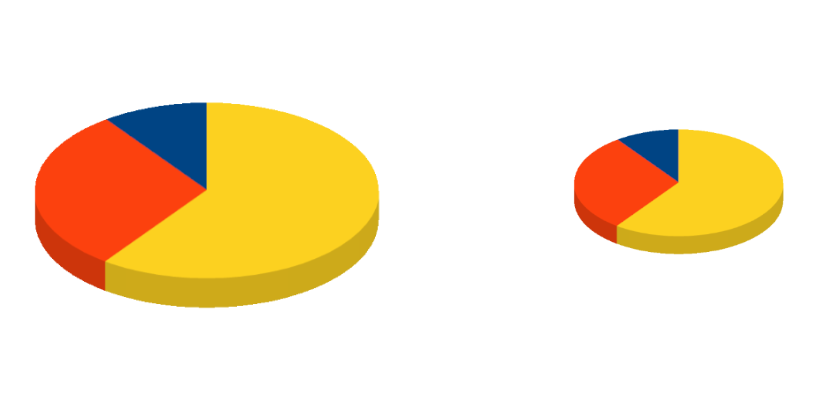
\includegraphics[scale=0.42]{base/pie_chat_01}
				};
			\end{scope}
			\node[align=left] at ($(graph1.west)+(4cm, -1.4cm)$) {
				\small A\\
				\small 60\%
			};
			\node[align=left] at ($(graph1.west)$) {
				\small B\\
				\small 30\%
			};
			\node[align=left] at ($(graph1.west)+(2cm, 1.5cm)$) {
				\small C\\
				\small 10\%
			};
			\node (pop) at ($(graph1.south)+(-2.5cm,-0.2cm)$) {
				\Large POPULAÇÃO
			};
			\node[align=left] at ($(graph1.east)$) {
				\small A\\
				\small 60\%
			};
			\node[align=left] at ($(graph1.east)+(-2.8cm, 0.95cm)$) {
				\small B\\
				\small 30\%
			};
			\node[align=left] at ($(graph1.east)+(-1.8cm, 1.25cm)$) {
				\small C\\
				\small 10\%
			};
			\node (pop) at ($(graph1.south)+(3.1cm,1cm)$) {
				AMOSTRA
			};
			
			\begin{scope}[local bounding box=title]
				\node[draw, align=center] at (1.5cm, 2.4cm){
					Estratificação\\
					Proporcional
				};
			\end{scope}
			\draw[
		        -triangle 90,
	        	line width=2mm,
	        	color=ocre!60,
	        	postaction={draw, line width=0.6cm, shorten >=0.4cm, -}
	    		] ($(title.south west)+(-0.5cm, -1.4cm)$) -- ($(title.south east)+(-1.2cm,-1.4cm)$);
	    	
		\end{tikzpicture}
	\end{pageWidthAreaPicture}
\end{pageWidthArea}

\begin{example}
	\label{example:amostra_estratificada_teste_droga}
	Com o objetivo de estudar a eficácia de uma determinada droga, vamos realizar um levantamento por amostragem estratificada proporcional de tamanho 10. Suponha que a população é composta por 10 drogas do laboratório A, 10 do laboratório B e 30 do laboratório C (Tabela \ref{table:composicao_example_amostra_estratificada_teste_droga}). A determinação do tamanho da amostra em cada estrato pode ser feita com porcentagem simples (Tabela \ref{table:tamanho_example_amostra_estratificada_teste_droga}). \\
	
	Assim, utilizando a Tabela de Números Aleatórios, de acordo com a primeira linha, tem-se
	\begin{center}
		\emphasis{9}, \emphasis{8}, 0, 8, $\dots$
	\end{center}
	donde, para o Laboratório A, escolhe-se $A_8$ e $A_9$. De acordo com a segunda linha,
	\begin{center}
		\emphasis{3}, 3, \emphasis{1}, 8, $\dots$
	\end{center}
	donde, para o Laboratório B, escolhe-se $B_3$ e $B_1$. Pela terceira linha,
	\begin{center}
		80, 95, \emphasis{10}, \emphasis{04}, \emphasis{06}, 96, 38, \emphasis{27}, \emphasis{07}, 74, \emphasis{20}, $\dots$
	\end{center}
	retirando a amostra $C_{10}$, $C_{04}$, $C_{06}$, $C_{27}$, $C_{07}$, $C_{20}$. Portanto, a amostra final será
	\begin{center}
		$\{A_8$, $A_9$, $B_1$, $B_3$, $C_{04}$, $C_{06}$, $C_{07}$, $C_{10}$, $C_{20}$, $C_{27}\}$
	\end{center}
\end{example}

\begin{sidepicture}{12cm}{table}{Composição da população do Exemplo \ref{example:amostra_estratificada_teste_droga}}
	\label{table:composicao_example_amostra_estratificada_teste_droga}
	\begin{tabular}{rl}\\\toprule
		Lab. A & $A_1$, $\dots$, $A_{10}$ \\
		Lab. B & $B_1$, $\dots$, $B_{10}$ \\ 
		Lab. C & $C_1$, $\dots$, $C_{10}$, $\dots$, $C_{30}$ \\ \bottomrule
	\end{tabular}
\end{sidepicture}

\begin{sidepicture}{8cm}{table}{Determinando o tamanho da amostra em cada estrato do Exemplo \ref{example:amostra_estratificada_teste_droga}}
	\label{table:tamanho_example_amostra_estratificada_teste_droga}
	\begin{tabular}{ccc}\\\toprule
		\small Estrato & \begin{tabular}{c}\small Proporção\\\small na\\\small População\end{tabular} & \begin{tabular}{c}\small Tamanho\\\small Amostral\\\small no\\\small Estrato\end{tabular}\\ \midrule
		\small Lab. A & \small $\dfrac{10}{50}=0,2$\vspace{10pt} & \small $0,2\cdot 10=2$ \\
		\small Lab. B & \small $\dfrac{10}{50}=0,2$\vspace{10pt} & \small $0,2\cdot 10=2$ \\ 
		\small Lab. C & \small $\dfrac{30}{50}=0,6$\vspace{10pt} & \small $0,6\cdot 10=6$ \\ \midrule
		\small Total & \small $\dfrac{50}{50}=1$ & \small $10$ \\ \bottomrule
	\end{tabular}
\end{sidepicture}

\subsection{Uma Fórmula para o Cálculo do Tamanho de Uma Amostra Aleatória Simples}

Seja $N$ o tamanho da população, $n$ o tamanho da amostra, $n_0$ uma primeira aproximação para o tamanho da amostra e $E_0$ o erro amostral tolerável.

Um primeiro cálculo do tamanho da amostra pode ser feito, mesmo sem conhecer o tamanho da população através de:
\begin{equation}
	n_0=\frac{1}{E_0^2}\text{.}
\end{equation}

Conhecendo o tamanho $N$ da população, podemos corrigir o cálculo acima por
\begin{equation}
	n=\frac{N\cdot n_0}{N+n_0}\text{.}
\end{equation}

\begin{remark}
	Perceba que quando $N\to\infty$, o valor de $n_0\to n$.
\end{remark}

\begin{example}
	Planeja-se um levantamento por amostragem para avaliar diversas características da população das 200 famílias moradoras de um bairro. Qual deve ser o tamanho mínimo de uma amostra aleatória simples, tal que, possamos admitir, com alta confiança, que os erros amostrais não ultrapassem 4\%.\\
	
	O cálculo inicial é
	\[
		n_0=\frac{1}{0,04^2}=625\text{,}
	\]
	podendo ser corrigido por
	\[
		n=\frac{200\cdot 625}{200+625}=152\text{,}
	\]
	ou seja, o tamanho mínimo de uma amostra aleatória simples deve ser 152 famílias para que os erros amostrais não ultrapassem 4\%.\\
	
	Perceba que para uma população de 200.000, o cálculo é extremamente parecido, inclusive, $n_0$ terá o mesmo valor e
	\[
		n=\frac{200.000\cdot 625}{200.000+625}=623\text{.}
	\]
\end{example}

\begin{note}{Arredondamentos}
	Uma observação a ser feita é que não se deve reduzir ou truncar a aproximação. Use sempre o próximo inteiro de modo a garantir que esteja dentro da margem de erro desejada.
\end{note}

\section{Distribuição de Frequências}

Quando se estuda uma variável, o maior interesse do pesquisador é conhecer a sua distribuição, ou seja, o comportamento dessa variável.

\section{Medidas de Tendência Central e de Dispersão}

Os dados, apresentados em tabelas e gráficos, constituem a base de toda a informação. Mas, às vezes, é preciso resumir essa informação. Usam-se então as medidas de tendência central, que \emphasis{dão o(s) valor(es) em torno do qual os dados se distribuem}. Sabe-se, porém, que as medidas de tendência central são tanto mais apropriadas para descrever um conjunto de dados quanto \emphasis{menor for a dispersão}. Então, também é necessário e importante estudar as medidas de dispersão.

Dentre as medidas de "\emphasis{tendências centrais}" destacamos:
\begin{itemize}
	\item A média.
	\item A mediana.
	\item A moda.
\end{itemize}

Dentre as medidas de "\emphasis{dispersão} destacamos:
\begin{itemize}
	\item A amplitude.
	\item A variância.
	\item O desvio-padrão.
	\item O coeficiente de variação.
\end{itemize}

\subsection{Medidas de Tendência Central}

\subsubsection{Média Aritmética para Dados não Agrupados}

A média aritmética para dados não agrupados é o quociente da divisão da soma dos valores da variável pelo número total dos valores dessa variável.
\[
	\overline{x} = \frac{\displaystyle\sum_{i=1}^{n} x_i}{n}
	\text{,}
\]
onde $x_i$ são os valores da variável e $n$ é o número de valores dessa variável.

\begin{example}
	\label{example:pesos_bezerros}
	O peso ao nascer de 7 bezerros machos da raça Charolesa em quilogramas são os seguintes: 47, 34, 45, 28, 37, 40, 42. A média desses pesos é
	\[
		\overline{x}=\frac{47+34+45+28+37+40+42}{7}=39\text{,}
	\]
	logo a média dos pesos dos bezerros é de 39kg.
\end{example}

\subsubsection{Desvio em Relação à Média}

O desvio em relação à média é a diferença entre cada elemento de um conjunto de dados e a média aritmética, isto é,
\[
	d_i=x_i-\overline{x}\text{.}
\]

\begin{example}
	\label{example:pesos_bezerros_desvios}
	Do Exemplo \ref{example:pesos_bezerros}, tem-se os desvios, dados por $d_i=x_i-\overline{x}$,
	\begin{itemize}
		\item $d_1=47-39=8$.
		\item $d_2=34-39=-5$.
		\item $d_3=45-39=6$.
		\item $d_4=28-39=-11$.
		\item $d_5=37-39=-2$.
		\item $d_6=40-39=1$.
		\item $d_7=42-39=3$.
	\end{itemize}
\end{example}

A soma dos desvios em relação à média é sempre nula. Do Exemplo \ref{example:pesos_bezerros_desvios}, tem-se
\[
	\sum_{i=1}^{7}d_i = 8-5+6-11-2+1+3=0\text{.}
\]

\begin{theorem}
	Somando-se (ou subtraindo-se) uma constante $c$ de todos os valores de um conjunto de dados, a média desse novo conjunto de dados fica aumentada (ou diminuída) dessa contante. Ou seja, se
	\[
		y_i=x_i\pm c\text{,}
	\]
	tem-se que
	\[
		\overline{y}=\overline{x}\pm c\text{.}
	\]
\end{theorem}

\begin{example}
	Somando uma constante 2 a cada um dos valores do conjunto de dados do Exemplo \ref{example:pesos_bezerros}, tem-se um novo conjunto dado por: 49, 36, 47, 30, 39, 42 e 44, e uma nova média dada por
	\[
		\overline{y}=\frac{49+36+47+30+39+42+44}{7}=41\text{.}
	\]
	
	Assim, vale que
	\[
		\overline{y}=\overline{x}+2=39+2=41\text{,}
	\]
	Ou seja, a nova média é 41 kg.
\end{example}

\begin{theorem}
	Multiplicando-se (ou dividindo-se) todos os valores de um conjunto de dados por uma constante $c$, a média desse novo conjunto de dados fica multiplicada (ou dividida) por essa constante. Ou seja, se
	\[
		y_i=x_i\cdot c\text{,}
	\]
	então, tem-se
	\[
		\overline{y}=\overline{x}\cdot c\text{.}
	\]
	
	Ainda, se
	\[
		y_i=\frac{x_i}{c}\text{,}
	\]
	tem-se
	\[
		\overline{y}=\frac{\overline{x}}{c}\text{.}
	\]
\end{theorem}

\begin{example}
	Multiplicando por 3 cada um dos valores do conjunto de dados do Exemplo \ref{example:pesos_bezerros}, tem-se um novo conjunto dado por: 141, 102, 135, 84, 111, 120 e 126 e uma nova média dada por
	\[
		\overline{y}=\frac{141+102+135+84+111+120+126}{7}=117\text{.}
	\]
	
	Assim, tem-se que
	\[
		\overline{y}=\overline{x}\cdot 3=39\cdot 3=117
		\text{,}
	\]
	portanto, a nova média é de 117 kg.
\end{example}

\subsubsection{Média Aritmética para Dados Agrupados Sem Intervalo de Classe}

Neste caso, como as frequências $f_i$ são números indicadores da intensidade de cada valor da variável, elas funcionam como fatores de ponderação, o que nos leva a calcular a \emphasis{média aritmética ponderada}, dada por
\[
	\overline{x}=\frac{
		\displaystyle \sum_{i=1}^{k} x_i f_i
	}{
		\displaystyle \sum_{i=1}^{n} f_i
	}
	= \frac{
		\displaystyle \sum_{i=1}^{k} x_i f_i
	}{
		n
	}
	\text{,}
\]
onde $k$ é o número de classes.

{\color{red}Fazer Exemplo Aqui.}

\subsubsection{Média Aritmética para Dados Agrupados com Intervalo de Classe}

Neste caso, "\emphasis{convencionamos}" que todos os valores incluídos em um determinado intervalo de classe sejam representados pelo seu \emphasis{ponto médio} ($x^{*}$), e determinamos a média aritmética ponderada através de:
\[
	\overline{x}=\frac{	
		\displaystyle \sum_{i=1}^{k} x_i^{*} f_i
	}{
		\displaystyle \sum_{i=1}^{k} f_i
	}
	= \frac{
		\displaystyle \sum_{i=1}^{k} x_i^{*} f_i
	}{
		n
	}
	\text{,}
\]
onde $k$ é o número de classes.

{\color{red}Fazer Exemplo Aqui.}

\subsection{Mediana}

A mediana é o \emphasis{valor central} que divide um conjunto de "\emphasis{dados ordenados}" ao meio, deixando 50\% dos valores dos dados a sua esquerda e 50\% à sua direita.

{\color{red}Fazer Exemplo Aqui.}

\subsection{Moda}

Denominamos por moda o valor que ocorre com maior frequência em um conjunto de dados.

{\color{red}Fazer Exemplo Aqui.}

\subsection{Qual a Melhor Medida de Centralidade?}

Não há uma única melhor resposta para esta questão, porque não há critérios objetivos para a determinação da medida mais representativa para todos os conjuntos de dados. As diferentes medidas de centralidade tem diferentes vantagens e desvantagens, algumas das quais estão resumidas no Quadro \ref{quadro:comparacao_medida_tc}.\\

\begin{pageWidthArea}
	\begin{pageWidthAreaPicture}{frame}{Comparação entre as medidas de tendências centrais.}
		\label{quadro:comparacao_medida_tc}
		\hspace{-15pt}
		\resizebox{\textwidth}{!}{%
		\begin{tabular}{|c|c|c|c|c|c|}
			\hline
			Medida & Uso & Existência & \begin{tabular}[c]{@{}c@{}}Leva em\\conta todos\\os valores\end{tabular} & \begin{tabular}[c]{@{}c@{}}Afetada\\por\\Outliers\end{tabular} & Vantagens\\ \hline
			Média & "Exagerado" & Sempre & Sim & Sim & \begin{tabular}[c]{@{}c@{}}Funciona bem\\com muitos\\métodos\\estatísticos.\end{tabular}\\ \hline
			Mediana & Comumente & Sempre & Não & Não & \begin{tabular}[c]{@{}c@{}}Sempre uma\\boa escolha\\na presença\\de \textit{outliers}.\end{tabular}\\ \hline
			Moda & Raramente & \begin{tabular}[c]{@{}c@{}}Pode não\\existir ou ter\\mais de uma\end{tabular} & Não & Não & \begin{tabular}[c]{@{}c@{}}Apropriada\\para dados\\nominais.\end{tabular}\\ \hline
		\end{tabular}
		}
	\end{pageWidthAreaPicture}
\end{pageWidthArea}

\begin{remark}
	Para um conjunto de dados unimodal que é aproximadamente simétrico, a média, a mediana e a moda são muito próximas.
\end{remark}

\begin{remark}
	Para um conjunto de dados obviamente assimétrico, seria melhor informar tanto a média como a mediana.
\end{remark}

{\color{red}Fazer exemplos aqui.}

\section{Medidas de Dispersão}

\subsection{Amplitude Total}

A amplitude total é a diferença entre os valores extremos do conjunto de dados.

{\color{red}Fazer exemplos aqui.}

Embora a amplitude total seja a medida de dispersão mais simples, existem várias restrições ao seu uso devido a sua instabilidade, uma vez que, ela utiliza somente os valores extremos do conjunto de dados, sendo extremamente sensível à presença de valores extremos (outliers). Neste caso, precisamos de uma medida que foge a essa "falha", isto é, que leva em consideração todos os valores de um conjunto de dados.

\subsection{Variância}

A variância é uma medida de variação de todos os valores de um conjunto de dados em torno de sua média, calculadas por
\begin{equation}
	\label{eqn:variancia_populacao}
	\sigma ^2 = \frac{
		\displaystyle \sum_{i=1}^{n} (x_i - \overline{x})^2
	} {
		n
	} \text{.}
\end{equation}

Desse modo, a variância é definida como a soma dos quadrados dos desvios, dividida por $n$. A Fórmula \ref{eqn:variancia_populacao} é chamada de \emphasis{Variância para População}.

Prova-se, no entanto, que para ter propriedades estatísticas desejáveis, é preciso que ese valor seja multiplicado pelo fator de correção
\[
	\frac{n}{n-1}
	\text{.}
\]

Dessa forma, a variância pode ser reescrita como
\begin{equation}
	\label{eqn:variancia_amostras}
	S^2=\frac{
		\displaystyle \sum_{i=1}^{n} (x_i - \overline{x})^2
	} {
		n-1
	}\text{.}
\end{equation}

A Fórmula \ref{eqn:variancia_amostras} é chamada de \emphasis{Variância para Amostras}. É possível desenvolver essa fórmula, algebricamente, de onde tira-se que
\[
	S^2=\frac{
		\displaystyle \sum_{i=1}^{n} x_i^2
		-
		\displaystyle \frac{
			\left (
				\displaystyle \sum_{i=1}^{n} x+i
			\right ) ^2
		}{n}
	} {
		n-1
	}
	\text{.}
\]

{\color{red}Fazer exemplos aqui.}

A variância tem a desvantagem de apresentar unidade de medida igual ao quadrado da unidade de medida dos dados. Dessa forma surge a necessidade de se extrair a raiz quadrada da variância, definindo assim o \emphasis{Desvio-Padrão}.

\subsection{Desvio-Padrão}

O desvio-padrão é a raiz quadrada positiva da variância. O desvio-padrão tem a vantagem de ter a mesma unidade de  medida dos dados.

{\color{red}Fazer exemplos aqui.}

\begin{theorem}
	Somando-se (ou subtraindo-se) uma constante $c$ de todos os valores de um conjunto de dados, o desvio-padrão não se altera. Isto é, se
	\[
		y_i=x_i\pm c\text{,}
	\]
	então,
	\[
		S_y=S_x\text{.}
	\]
\end{theorem}

\begin{theorem}
	Multiplicando-se todos os valores de um conjunto de dados por uma constante $c\neq 0$, o desvio-padrão fica multiplicado por essa constante. Isto é, se
	\[
		y_i=x_i\cdot c\text{,}
	\]
	então,
	\[
		S_y=c\cdot S_x\text{.}
	\]
\end{theorem}

Tanto a variância quanto o desvio padrão são medidas que fornecem informações complementares à informação contida na média.

{\color{red}Fazer exemplo aqui.}

%\subsection{Teorema de Chebyshev}


\chapter{Introdução à Probabilidade}

Em probabilidade, estudam-se os experimentos aleatórios. Assim, primeiro, é necessário definir um experimento aleatório, diferenciando o mesmo de um experimento determinístico.

\begin{definition}
	Os \emphasis{Experimentos Determinísticos} são experimentos que ao serem repetidos "nas mesmas condições" conduzem ao mesmo resultado.
\end{definition}

\begin{example}
	Se aquecermos a água a 100 $^{\text{o}}$C, ela entrará em ebulição.
\end{example}

\begin{definition}
	Os \emphasis{Experimentos Aleatórios} são experimentos que ao serem repetidos "nas mesmas condições" em geral, não produzem o mesmo resultado.
\end{definition}

\begin{example}
	São exemplos de experimentos aleatórios:
	\begin{itemize}
		\item O número de grãos produzidos por hectares;
		\item Tipos de cultivares de milho;
		\item Tempo de uma reação química;
		\item Peso de um animal.
	\end{itemize}
\end{example}

\section{Espaço Amostral e Eventos}

\begin{definition}
	Denominaremos espaço amostral associado a um experimento ($E$) o conjunto de seus possíveis resultados, que representaremos por $S$, cujos elementos serão denominados eventos simples ou pontos amostrais.
\end{definition}

\begin{example}
	Seja o experimento $E$: Lançamento de uma moeda. Então, $S=\{C,\text{ }K\}$, onde $C$ representa cara e $K$ coroa.
\end{example}

\begin{example}
	\label{example:pecas_boas_defeituosas}
	Seja o experimento $E$: três peças são retiradas de uma linha de produção e classificadas em Boa ($B$) ou Defeituosas ($D$). Assim,
	\[
		S=\{BBB, BBD, BDB, DBB, BDD, DBD, DDB, DDD\}\text{.}
	\]
\end{example}

\begin{example}
	Seja o experimento $E$: número de plantas doentes em um tomateiro. Então,
	\[
		S=\{0, 1, 2, \dots, n\}\text{,}
	\]
	onde $n$ é o número máximo de plantas neste tomateiro.
\end{example}

\begin{example}
	Seja $E$: uma moeda é lançada sucessivamente até que ocorra cara pela primeira vez. Assim,
	\[
		S=\{C, KC, KKC, KKKC, KKKKC, \dots \}\text{.}
	\]
\end{example}

\begin{example}
	Seja $E$: tempo de vida de um animal. Então,
	\[
		S=\{t\in\mathbb{R}/ t\geqslant 0\}\text{,}
	\]
	ou
	\[
		S=\mathbb{R}_{+}\text{.}
	\]
\end{example}

\begin{definition}
	Denominaremos de evento a todo resultado ou subconjunto de resultados de um experimento.
\end{definition}

\begin{remark}
	Eventos simples são representados por um conjunto unitário.
\end{remark}

\begin{remark}
	Diremos que um evento $A$ ocorre quando o resultado do experimento é um evento simples pertencente ao evento $A$.
\end{remark}

\begin{example}
	Consideremos o Exemplo \ref{example:pecas_boas_defeituosas} e, seja um evento $A$: "Duas peças são boas". Tem-se
	\[
		A=\{BBD, BDB, DBB\}\text{,}
	\]
	onde $B$: Boa e $D$: Defeituosa. Então, $A$ ocorre se um dos três eventos simples:
	\begin{center}
		$BBD$, $BDB$, $DBB$,
	\end{center}
	ocorrer.
\end{example}

\begin{example}
	Considere o lançamento de duas moedas e, seja o evento B: "o número de caras é igual ao número de coroas". Assim,
	\[
		B=\{CK, KC\}\text{,}
	\]
	onde $C$: cara e $K$: coroa.
\end{example}


\nosidepicturearea
\part{Inferência Estatística}

%----------------------------------------------------------------------------------------
%	CHAPTER 1
%----------------------------------------------------------------------------------------

\chapterimage{heading_var_aleatoria} % Chapter heading image
\opensidepicturearea

\chapter{Variável Aleatória Contínua}

\nocite{livro_bussab_morettin}
Considere a distribuição de probabilidade da variável aleatória discreta $X$, conforme a Tabela \ref{testlabel} e a Figura \ref{testlabel2}. As áreas dos retângulos da Figura \ref{testlabel2} são 
\[
	A_i = b_i\cdot h_i
	\text{,}
\]
onde $b_i$ indica a base e $h_i$ indica a altura, ou seja,
\[
	A_1 = b_1 \cdot h_1 = 1 \cdot 0,1 = 0,1 \Longrightarrow P(X=1)=A_1
	\text{,}
\]
\[
	A_2 = b_2 \cdot h_2 = 1 \cdot 0,2 = 0,2 \Longrightarrow P(X=2)=A_2
	\text{,}
\]
\[
	\vdots
\]
\[
	A_5 = b_5 \cdot h_5 = 1 \cdot 0,1 = 0,1 \Longrightarrow P(X=5)=A_5
	\text{.}
\]

\begin{sidepicture}{7cm}{table}{Distribuição de probabilidade da variável aleatória discreta $X$}
	\label{testlabel}
	\begin{tabular}{ccc}\\\toprule  
		$x$ & $P(X=x_i)$ \\ \midrule
		1 & 0,1 \\
		2 & 0,2 \\ 
		3 & 0,4 \\
		4 & 0,2 \\
		5 & 0,1 \\ \midrule
		Total & 1,0\\  \bottomrule
	\end{tabular}
\end{sidepicture}

\begin{sidepicture}{1cm}{picture}{Gráfico da distribuição de probabilidade da variável aleatória discreta $X$}
	\label{testlabel2}
	\resizebox{5.6cm}{!}{
		\begin{tikzpicture}
			\begin{axis}[
				axis x line=left,
				axis y line=left,
				ybar,
				enlargelimits=0.15,
				title={$P(X=x_i)$},
				symbolic x coords={1,2,3,4,5},
	    		xtick=data,
	    		bar width=20pt
		    ]
				\addplot[color=ocre, fill=ocre!30] coordinates {(1,0.1) (2,0.2) (3,0.4) (4,0.2) (5,0.1)};
			\end{axis}
		\end{tikzpicture}
	}
\end{sidepicture}

Ainda, somando todas as áreas, tem-se
\[
	\sum_{i=1}^{5} A_i = 1 = \sum_{i=1}^{5} P(X=x_i)
\]
onde é possível concluir que para calcular $P(1\leqslant X \leqslant 3)$ basta fazer $A_1 + A_2 + A_3$.
\newpage

\begin{sidepicture}{0cm}{picture}{Exemplo de curva que pode ser traçada unindo os pontos médios das bases superiores dos retângulos da Figura \ref{testlabel2}}
	\label{testlabel3}
		\begin{tikzpicture}
			\tkzInit[xmin=-0.5,xmax=3.4,ymin=-0.5,ymax=4]
			\tkzDrawX[noticks]
			\tkzDrawY[noticks, label={$P(X=x_i)$}]
			\tkzFct[domain=0.2:3.8, color=ocre, line width=2pt, samples=2000]{20 * (\gauss{4}{2}{2.2})-0.3}
			\tkzDrawArea[color=ocre!30, domain = 0.5:1.6]
			\tkzDefPointByFct(0.5)
			\tkzGetPoint{A}
			\tkzDefPointByFct(1.6)
			\tkzGetPoint{B}
			\tkzPointShowCoord[xlabel=$a$, xstyle={below=7pt}, noydraw](A)
			\tkzPointShowCoord[xlabel=$b$, xstyle={below=7pt}, noydraw](B)
			\tkzText[color=black](2,4.4) {$y=f(x)$}
		\end{tikzpicture}
\end{sidepicture}

Agora, tomando os pontos médios das bases superiores dos retângulos e ligando os mesmos por uma curva, tem-se uma função contínua $f(x)$, como a Figura \ref{testlabel3}.

\begin{definition}
	Uma variável aleatória $X$ é contínua\index{Variável Aleatória Contínua} em $\mathbb{R}$ se existir uma função $f(x)$ tal que:
	\begin{enumerate}[label={\roman*)}]
		\item $f(x) \geqslant 0$; e
		\item $\displaystyle \int_{-\infty}^{+\infty} f(x)dx = 1$.
	\end{enumerate}
	
	A função $f(x)$ é chamada função densidade de probabilidade\index{Função Densidade de Probabilidade}.
\end{definition}

\begin{remark}
	Para calcular $P(a\leqslant X \leqslant b)$, basta calcular a área delimitada por $f(x)$, eixo $x$ e pelas retas $x=a$ e $x=b$, isto é
	\begin{equation}
		P(a\leqslant x \leqslant b) = \int_{a}^{b} f(x)dx
		\text{.}
	\end{equation}
\end{remark}

\begin{remark}
	Sobre qualquer ponto individual a área será zero, isto é $P(X=x_i)=0$.
\end{remark}

\begin{remark}
	A igualdade nos extremos indifere no resultado, isto é,
	\begin{align*}
		P(a\leqslant X \leqslant b) &= P(a < X \leqslant b)\\
							  		 &=P(a\leqslant X < b)\\
									 &=P(a<X<b)\text{.}
	\end{align*}
\end{remark}

\begin{definition}
	A esperança\index{Esperança} de uma variável aleatória contínua é dada por
	\begin{equation}
		E(X)=\int_{-\infty}^{+\infty} xf(x)dx
		\text{.}
	\end{equation}
\end{definition}

\begin{definition}
	A mediana\index{Mediana} é o valor $Md$ que satisfaz $P(X\geqslant Md)=0,5$ e $P(X\leqslant Md)=0,5$.
\end{definition}

\begin{definition}
	A moda\index{Moda} é o valor $Mo$ tal que
	\begin{equation}
		f(Mo)=\max_x f(x)
		\text{.}
	\end{equation}
\end{definition}

\begin{definition}
	A variância\index{Variância} é dada por
	\begin{equation}
		Var(X)=\int_{-\infty}^{+\infty} (x-E(x))^2 f(x) dx
		\text{,}
	\end{equation}
	ou ainda,
	\begin{equation}
		Var(X)=E(X^2)-(E(X))^2
		\text{.}
	\end{equation}
\end{definition}

\begin{definition}
	A função de distribuição\index{Função de Distribuição Acumulada} ou densidade\index{Função de Densidade Acumulada} acumulada é definida por
	\begin{equation}
		F(x)=P(X\leqslant x)=\int_{-\infty}^{x} f(t)dt
		\text{.}
	\end{equation}
\end{definition}

\begin{sidepicture}{0cm}{picture}{Exemplo de gráfico de função de densidade acumulada}
	\label{testlabel4}
	\begin{tikzpicture}
		\tkzInit[xmin=-3,xmax=2.3,ymin=-0.5,ymax=3.2]
		\tkzDrawX[noticks]
		\tkzDrawY[noticks,label={$F(x)$}]
		\tkzFct[domain=-3:2.3,line width=2pt, color=ocre, samples=2000]{atan(2*x) + 1.5}
		\tkzHLine{3}
		\tkzText[color=black](-0.5,3) {1}
		\tkzText[color=black](-0.5,0) {0}
	\end{tikzpicture}
\end{sidepicture}

Um exemplo de gráfico de uma função de distribuição acumulada pode ser visto na Figura \ref{testlabel4}.

\begin{remark}
	Podemos obter a função densidade de probabilidade, se existir, a partir de $F(x)$ pois
	\[
		\frac{d}{dx}F(x) = f(x)
	\]
	nos pontos onde $F(x)$ é derivável.
\end{remark}

\begin{example}
	Verificar se
	\[
		f(x)= \begin{cases}
			2x+3, &\text{ se } 0<x\leqslant 2\\
			0, &\text{ se } x \leqslant 0 \text{ ou } x > 2
		\end{cases}
	\]
	é uma função densidade de probabilidade.
	
	Primeiro, precisamos que  $f(x)\geqslant 0$. Assim, $2x+3\geqslant 0$, ou seja $2x\geqslant -3$, onde se conclui que $x \geqslant -\frac{3}{2}$, logo, $f(x)\geqslant 0$, $\forall x\in \mathbb{R}$.
	
	Calculando
	\begin{align*}
		\int_{-\infty}^{+\infty} f(x) dx &= \int_{0}^{2} (2x + 3)dx = (x^2+3x)\Big|_{0}^{2} = 4 + 6\\
										  &= 10\text{.}
	\end{align*}
	
	Logo, $\displaystyle \int_{-\infty}^{+\infty} f(x)dx = 10 \neq 1$, logo, $f(x)$ não é função densidade de probabilidade.
\end{example}

\begin{remark}
	Perceba que se usarmos a função
	\[
		f(x)=\begin{cases}
			\dfrac{2x+3}{10}\text{,} &\text{ se } 0<x\leqslant 2\\
			0\text{,} & \text{ se } x\leqslant 0\text{ ou }x>2
		\end{cases}
	\]
	ela se torna uma função densidade de probabilidade pois passamos a ter
	\[
		\int_{-\infty}^{+\infty} f(x)dx = 1
		\text{.}
	\]
\end{remark}

\begin{sidepicture}{5cm}{picture}{Descrição 3}
	\label{testlabel5}
	\begin{tikzpicture}
		\tkzInit[xmin=-1.5,xmax=3,ymin=-0.5,ymax=2]
		\tkzDrawX[noticks]
		\tkzDrawY[noticks,label={$y=f(x)$}]
		\tkzDefPoint(-1.5,0){A}
		\tkzDefPoint(0,0){B}
		\tkzDefPoint(1,2){C}
		\tkzDefPoint(1,0){D}
		\tkzDefPoint(3,0){E}
		\tkzPointShowCoord[xlabel=$1$, xstyle={below=7pt}, ylabel=$2$, ystyle={left=7pt}](C)
		\tkzDrawSegment[color=ocre, line width=2pt](A,B)
		\tkzDrawSegment[color=ocre, line width=2pt](B,C)
		\tkzDrawSegment[color=ocre, line width=2pt](D,E)
		\tkzDrawPoint[fill=ocre, size=10](C)
		\tkzDrawPoint[fill=white, size=10](D)
		\tkzText(1.3, 1){$y=f(x)$}
	\end{tikzpicture}
\end{sidepicture}

\begin{pageWidthArea}
	\begin{example}
		\begin{multicols}{2}
			Considere a função
			\[
				f(x)=\begin{cases}
					kx\text{,}&\text{ se } 0 < x \leqslant 1\\
					0\text{,}&\text{ se } x\leqslant 0\text{ ou }x>1
				\end{cases}
				\text{,}
			\]
			onde podemos determinar
			\begin{enumerate}[label={(\alph*)}]
				\item o valor de $k$ afim de que $f(x)$ seja função densidade de probabilidade,
				\[
					\int_{-\infty}^{+\infty} f(x)dx=1
					\text{,}
				\]
				deste modo,
				\[
					\int_{0}^{1} kx dx = \frac{k}{2}x^2\Big|_{0}^{1}
									    = \frac{k}{2}
									    = 1\text{,}
				\]
				de onde conclui-se que $k=2$.
				
				\item o valor de $P(0\leqslant X\leqslant \frac{1}{2})$, dado pela integral
				\[
					\int_{0}^{\frac{1}{2}} 2x dx = x^2\Big|_{0}^{\frac{1}{2}}=\frac{1}{4}
					\text{.}
				\]
				\item a esperança $E(X)$, dada por
				\[
					E(X)=\int_{-\infty}^{+\infty}xf(x)dx
						=\int_{0}^{1}2x^2dx
						=\frac{2}{3}
					\text{.}
				\]
				
				\item A variância, $Var(X)$, é calculada como
				\[
					Var(X)=\int_{-\infty}^{+\infty} (x-E(X))^2 f(x) dx
					\text{,}
				\]
				ou seja,
				\begin{align*}
					Var(X) &=\int_{-\infty}^{+\infty} (x - E(X))^2 f(x) dx\\
						   &=\int_{0}^{1} \left (x-\frac{2}{3} \right )^2 2xdx = \cdots\\
						   &=\frac{1}{2}-\frac{8}{9}+\frac{4}{9} = \frac{1}{18}
						   \text{.}
				\end{align*}
				
				\item a função de densidade acumulada pode ser calculada como
				\[
					F(x)=\int_{-\infty}^{x} f(t)dt
					\text{,}
				\]
				deste modo, tem-se que dividir em três casos, sendo que quando $x\leqslant 0$, $F(x)=0$, quando $x>1$, $F(x)=1$ e, quando $0<x\leqslant 1$,
				\[
					F(x)=\int_{-\infty}^{0} 0dt + \int_{0}^{x}2tdt=x^2\text{.}
				\]
				de onde a função $F(x)$ é
				\[
					F(x)=\begin{cases}
						0\text{,}&\text{ se } x \leqslant 0\\
						x^2\text{,}&\text{ se } 0<x\leqslant 1\\
						1\text{,}&\text{ se } x > 1
					\end{cases}
					\text{.}
				\]
				
				\item o gráfico de $f(x)$ e $F(x)$ estão nas Figuras \ref{testlabel5} e \ref{testlabel6}, respectivamente.
			\end{enumerate}	
		\end{multicols}
	\end{example}
\end{pageWidthArea}

\begin{example}
	\label{ex:cap0:temp_eq_eletric}
	Seja $X:$"tempo durante o qual um equipamento elétrico é usado em carga máxima, num certo período de tempo, em minutos". A função densidade de probabilidade de $X$ é dada por
	\[
		f(x)=\begin{cases}
			\frac{1}{1500^2}x\text{,}&\text{ se } 0 \leqslant x < 1500\\
			\frac{1}{1500^2}(3000-x)\text{,}&\text{ se } 1500\leqslant x \leqslant 3000
		\end{cases}
		\text{.}
	\]
	
	Calcule o tempo médio em que o equipamento será utilizado em carga máxima.
	
	Para calcular o tempo médio, devemos calcular a esperança
	\begin{align*}
		E(X)&=\int_{0}^{1500} \frac{1}{1500^2}x^2dx
			 +\int_{1500}^{3000}\frac{1}{1500^2}(3000x-x^2)dx\\
			&=\frac{1}{1500^2}\cdot \frac{1}{3}x^3\Big|_{0}^{1500}
			 +\frac{1}{1500^2}\left (\frac{3000x^2}{2} - \frac{x^3}{3} \right ) \Big|_{1500}^{3000}\\
			&=1500\text{,}
	\end{align*}
	ou seja, o tempo médio em que o equipamento será utilizado em carga máxima é de 1500 minutos. O gráfico da função $f(x)$ pode ser visto na Figura \ref{fig:cap0:curva_fdp_ex_eq_eletric}.
\end{example}

\begin{sidepicture}{10cm}{picture}{Descrição 3}
	\label{testlabel6}
	\begin{tikzpicture}
		\tkzInit[xmin=-1.5,xmax=3,ymin=-0.5,ymax=2]
		\tkzDrawX[noticks]
		\tkzDrawY[noticks,label={$y=F(x)$}]
		\tkzDefPoint(-1.5,0){A}
		\tkzDefPoint(0,0){B}
		\tkzDefPoint(1,1){C}
		\tkzDefPoint(3,1){D}
		\tkzPointShowCoord[xlabel=$1$, xstyle={below=7pt}, ylabel=$1$, ystyle={left=7pt}](C)
		\tkzFct[color=ocre, line width=2pt, domain=0:1]{x**2}
		\tkzDrawSegment[color=ocre, line width=2pt](A,B)
		\tkzDrawSegment[color=ocre, line width=2pt](C,D)
		\tkzText[color=black](2, 1.7){$y=F(x)$}
	\end{tikzpicture}
\end{sidepicture}

\begin{sidepicture}{5cm}{picture}{Gráfico da função de densidade de probabilidade do Exemplo \ref{ex:cap0:temp_eq_eletric}}
	\label{fig:cap0:curva_fdp_ex_eq_eletric}
	\begin{tikzpicture}
		\tkzInit[xmin=-0.5,xmax=3,ymin=-0.5,ymax=2]
		\tkzDrawX[noticks]
		\tkzDrawY[noticks,label={$y=f(x)$}]
		\tkzDefPoint(0,0){A}
		\tkzDefPoint(1.5,0.5){B}
		\tkzDefPoint(3,0){C}
		\tkzPointShowCoord[xlabel=$1500$, xstyle={below=7pt}, ylabel=$\frac{1}{1500}$, ystyle={left=7pt}](B)
		\tkzDrawSegment[color=ocre, line width=2pt](A,B)
		\tkzDrawSegment[color=ocre, line width=2pt](B,C)
	\end{tikzpicture}
\end{sidepicture}

\section{Modelo Uniforme Contínuo}\index{Modelo Uniforme Contínuo}

Uma variável aleatória $X$ tem distribuição uniforme\index{Distribuição Uniforme} de probabilidade no intervalo $[a,b]$ se a sua função densidade de probabilidade é dada por
\[
	f(x)=\begin{cases}
		k\text{,}&\text{ se } a\leqslant x \leqslant b\\
		0\text{,}&\text{ se } x < a\text{ ou }x>b
	\end{cases}
	\text{.}
\]

A notação utilizada aqui será $X \sim U[a,b]$. Uma representação gráfica de $f(x)$ é apresentada na Figura \ref{fig:cap0:modelo_uniforme_continuo}.

O valor de $k$ pode ser facilmente calculado pois $\displaystyle\int_a^b kdx = 1$, ou seja, $kx\Big|_a^b=1$, de onde $k=\dfrac{1}{b-a}$, logo
\[
	f(x)=\begin{cases}
		\dfrac{1}{b-a}\text{,}&\text{ se } a\leqslant x\leqslant b\\
		0\text{,}&\text{ se }x<a\text{ ou }x>b
	\end{cases}
	\text{.}
\]

\begin{sidepicture}{8cm}{picture}{Gráfico da função $f(x)$ do modelo uniforme contínuo}
	\label{fig:cap0:modelo_uniforme_continuo}
	\begin{tikzpicture}
		\tkzInit[xmin=-1,xmax=4,ymin=-0.5,ymax=2]
		\tkzDrawX[noticks]
		\tkzDrawY[noticks,label={$f(x)$}]
		\tkzDefPoint(-1,0){A}
		\tkzDefPoint(1,0){B}
		\tkzDefPoint(1,1){C}
		\tkzDefPoint(3,1){D}
		\tkzDefPoint(3,0){E}
		\tkzDefPoint(4,0){F}
		\tkzPointShowCoord[xlabel=$a$, xstyle={below=7pt}, ylabel=$k$, ystyle={left=7pt}](C)
		\tkzPointShowCoord[xlabel=$b$, xstyle={below=7pt}, noydraw](D)
		\tkzDrawSegment[color=ocre, line width=2pt](A,B)
		\tkzDrawSegment[color=ocre, line width=2pt](C,D)
		\tkzDrawSegment[color=ocre, line width=2pt](E,F)
		\tkzDrawPoint[fill=ocre, size=10](C)
		\tkzDrawPoint[fill=ocre, size=10](D)
		\tkzDrawPoint[fill=white, size=10](B)
		\tkzDrawPoint[fill=white, size=10](E)
	\end{tikzpicture}
\end{sidepicture}

\begin{example}
	\label{ex:ponto_entre_0_2}
	Um ponto é escolhido ao acaso no intervalo $[0,2]$. Qual a probabilidade de que esteja entre 1 e 1,5?.\\
	
	Primeiro, perceba que, como o modelo adotado é o uniforme, a função $f(x)$ será dada por
	\[
		f(x)=\begin{cases}
			\dfrac{1}{2}\text{,}&\text{ se }0\leqslant x\leqslant 2\\
			0\text{,}&\text{ se } x<0\text{ ou }x>2
		\end{cases}\text{.}
	\]
	
	Deste modo, calculando a probabilidade de que esteja entre 1 e 1,5, tem-se
		\begin{align*}
			P(1<X<1,5)&=\int_{1}^{1,5} \frac{1}{2} dx\\
					  &=\frac{1}{2}\Big|_{0}^{1,5}\\
					  &=\frac{1,5}{2}-\frac{1}{2}\\
					  &=\frac{1}{4}\text{.}
		\end{align*}
\end{example}

A função distribuição (acumulada) de $X$, cuja representação gráfica está na Figura \ref{fig:cap0:modelo_uniforme_continuo_acumulada}, é dada por
\[
	F(x)=\begin{cases}
		0\text{,}&\text{ se }x\leqslant a\\
		\dfrac{x-a}{b-a}\text{,}&\text{ se }a<x<b\\
		1\text{,}&\text{ se }x\geqslant b
	\end{cases}
	\text{.}
\]

\begin{sidepicture}{2cm}{picture}{Gráfico da função $F(x)$ do modelo uniforme contínuo}
	\label{fig:cap0:modelo_uniforme_continuo_acumulada}
	\begin{tikzpicture}
		\tkzInit[xmin=-1,xmax=4,ymin=-0.5,ymax=2]
		\tkzDrawX[noticks]
		\tkzDrawY[noticks,label={$f(x)$}]
		\tkzDefPoint(-1,0){A}
		\tkzDefPoint(1,0){B}
		\tkzDefPoint(3,1){C}
		\tkzDefPoint(4,1){D}
		\tkzPointShowCoord[xlabel=$a$, xstyle={below=7pt}, noydraw](B)
		\tkzPointShowCoord[xlabel=$b$, xstyle={below=7pt}, ylabel=$1$, ystyle={left=7pt}](C)
		\tkzDrawSegment[color=ocre, line width=2pt](A,B)
		\tkzDrawSegment[color=ocre, line width=2pt](B,C)
		\tkzDrawSegment[color=ocre, line width=2pt](C,D)
	\end{tikzpicture}
\end{sidepicture}

A esperança $E(X)$ e a variância $Var(X)$ são, respectivamente
\begin{equation}
	E(X)=\frac{b+a}{2}
	\text{.}
\end{equation}
\begin{equation}
	Var(X)=\frac{(b-a)^2}{12}
	\text{.}
\end{equation}

\begin{example}
	Considere o Exemplo \ref{ex:ponto_entre_0_2} e determine os valores de $E(X)$ e $Var(X)$.\\
			
	A esperança será
		\begin{align*}
			E(X)&=\frac{b+a}{2}\\
				&=\frac{2+0}{2}\\
				&=1\text{.}
		\end{align*}
		
	A variância será
		\begin{align*}
			Var(X)&=\frac{(b-a)^2}{12}\\
				  &=\frac{(2-0)^2}{12}\\
				  &=\frac{4}{12}\\
				  &=\frac{1}{3}\text{.}
		\end{align*}
\end{example}

\begin{example}
	A dureza $H$ de uma peça de aço pode ser pensada como sendo uma variável aleatória com distribuição uniforme no intervalo $[50, 70]$. \\
	
	Perceba que a função de distribuição de probabilidade, para este exemplo, será
	\[
		f(x)=\begin{cases}
			\dfrac{1}{20}\text{,}&\text{ se } 50\leqslant x\leqslant 70\\
			0\text{,}&\text{ se } x<50\text{ ou }x>70
		\end{cases}\text{.}
	\]
	
	A probabilidade de que uma peça tenha dureza entre 55 e 60, isto é $P(55<X<60)$, pode ser determinado facilmente por
	\begin{align*}
		P(55<X<60)&=\int_{55}^{60} \frac{1}{20}dx\\
				  &=\frac{1}{20}x\Big|_{55}^{60}\\
				  &=\frac{60-55}{20}\\
				  &=\frac{1}{4}\text{.}
	\end{align*}
\end{example}

\section{Distribuição Exponencial}\index{Distribuição Exponencial}

Uma variável aleatória $X$ tem distribuição exponencial de probabilidade se a sua função densidade de probabilidade é dada por
\[
	f(x)=\begin{cases}
		\lambda e^{-\lambda x}\text{,}&\text{ se }x\geqslant 0\\
		0\text{,}&\text{ se }x<0
	\end{cases}
	\text{.}
\]

A notação utilizada aqui será $X\sim Exp(\lambda)$. O gráfico da função densidade de probabilidade é visto na Figura \ref{fig:cap0:modelo_exponencial}.

\begin{sidepicture}{2cm}{picture}{Gráfico da função densidade de probabilidade do modelo exponencial}
	\label{fig:cap0:modelo_exponencial}
	\begin{tikzpicture}
		\tkzInit[xmin=-0.5,xmax=2.5,ymin=-0.5,ymax=2.5]
		\tkzDrawX[noticks]
		\tkzDrawY[noticks,label={$f(x)$}]
		\tkzFct[domain=0:2.5, samples=2000, color=ocre, line width=2pt]{2*exp(-2*x)}
		\tkzDrawArea[color=ocre!30,domain = 0:2.5]
		\tkzText[color=black](-0.5,2.2){$\lambda$}
		\tkzDefPoint(-0.05,2){A}
		\tkzDrawPoint[fill=ocre, size=2](A)
	\end{tikzpicture}
\end{sidepicture}

\begin{remark}
	Perceba que a área delimitada pela curva $y=f(x)$ da Figura \ref{fig:cap0:modelo_exponencial} é sempre a mesma, independente do valor de $\lambda$, pois sua área é dada pela integral
	\[
		\int_{0}^{\infty} \lambda e^{-\lambda x}dx
		\text{,}
	\]
	que pode ser, facilmente, resolvida por substituição simples, resultando em
	\begin{align*}
		\int_{0}^{\infty} \lambda e^{-\lambda x}dx &= -e^{-\lambda x}\Big|_{0}^{\infty}\\ 
													&= \lim_{x\to \infty} (-e^{-\lambda x}) + e^0\\
													&=1
		\text{,}
	\end{align*}
	portanto a área delimitada pela curva $y=f(x)$ é, independente do valor de $\lambda$, igual a 1.
\end{remark}

\begin{example}
	\label{ex:exponencial_determine_k}
	Uma variável aleatória $X$ tem função densidade de probabilidade dada por
	\[
		f(x)=\begin{cases}
			\frac{k}{2}e^{-x}\text{,}&\text{ se }x\geqslant 0\\
			0\text{,}&\text{ se }x<0
		\end{cases}
		\text{.}
	\]
	
	O valor de $k$ pode ser determinado de duas formas. A primeira delas é, relembrando que para $x\geqslant 0$, $f(x)=\lambda e^{-\lambda x}$. Como, na função do exemplo, $-\lambda x=-x$, $\lambda=1$ e, portanto, $\frac{k}{2}=1$, de onde, naturalmente, $k=2$. Outra forma de se encontrar o valor de $k$ é resolvendo a equação
	\[
		\int_{0}^{\infty} \frac{k}{2}e^{-x}dx=1
		\text{,}
	\]
	que resultará, também, em $k=2$. Assim, a função, $f(x)$, cuja representação gráfica está na Figura \ref{fig:cap0:modelo_exponencial_exemplo_k}, passa a ser
	\[
		f(x)=\begin{cases}
			e^{-x}\text{,}&\text{ se }x\geqslant 0\\
			0\text{,}&\text{ se }x<0
		\end{cases}
		\text{.}
	\]
\end{example}

\begin{sidepicture}{0cm}{picture}{Gráfico da função densidade de probabilidade do Exemplo \ref{ex:exponencial_determine_k}.}
	\label{fig:cap0:modelo_exponencial_exemplo_k}
	\begin{tikzpicture}
		\tkzInit[xmin=-0.5,xmax=2.5,ymin=-0.5,ymax=2.5]
		\tkzDrawX[noticks]
		\tkzDrawY[noticks,label={$f(x)$}]
		\tkzFct[domain=0:2.5, samples=2000, color=ocre, line width=2pt]{exp(-x)}
		\tkzDrawArea[color=ocre!30,domain = 0:2.5]
		\tkzText[color=black](-0.5,1.2){1}
		\tkzDefPoint(-0.05,1){A}
		\tkzDrawPoint[fill=ocre, size=2](A)
	\end{tikzpicture}
\end{sidepicture}

A função distribuição acumulada, por sua vez, é calculada por
\begin{align*}
	F(x)&=\int_{0}^{x} \lambda e^{-\lambda t} dt\\
		&=-e^{-\lambda t}\Big|_{0}^{x}\\
		&=1-e^{-\lambda x}\text{,}
\end{align*}
ou seja, a função distribuição acumulada, cuja representação gráfica está na Figura \ref{fig:cap0:modelo_exponencial_acumulada}, é
\[
	F(x)=\begin{cases}
		1-e^{-\lambda x}\text{,}&\text{ se }x\geqslant 0\\
		0\text{,}&\text{ se }x<0
	\end{cases}
	\text{.}
\]

\begin{sidepicture}{0cm}{picture}{Gráfico da função distribuição acumulada do modelo exponencial}
	\label{fig:cap0:modelo_exponencial_acumulada}
	\begin{tikzpicture}
		\tkzInit[xmin=-0.5,xmax=2.5,ymin=-0.5,ymax=2.5]
		\tkzDrawX[noticks]
		\tkzDrawY[noticks,label={$F(x)$}]
		\tkzFct[domain=0:2.5, samples=2000, color=ocre, line width=2pt]{2*(1-exp(-2*x))}
		\tkzHLine{2}
		\tkzText[color=black](-0.5,2) {1}
	\end{tikzpicture}
\end{sidepicture}

\begin{example}
	Considere a variável aleatória $X$ e a função densidade de probabilidade $f(x)$ do Exemplo \ref{ex:exponencial_determine_k}. A função distribuição acumulada $F(x)$ para essa variável aleatória pode ser determinada, facilmente, utilizando
	\begin{align*}
		F(x)&=P(X\leqslant x)\\
			&=\int_{0}^{x}e^{-t}dt\\
			&=1-e^{-x}\text{,}
	\end{align*}
	de onde conclui-se que a função $F(x)$ é
	\[
		F(x)=\begin{cases}
			1-e^{-x}\text{,}&\text{ se } x \geqslant 0\\
			0\text{,}&\text{ se } x < 0
		\end{cases}
		\text{.}
	\]
	
	A mediana é um valor $Md$ tal que $P(X\leqslant Md)\geqslant 0,5$ e $P(X\geqslant Md)\geqslant 0,5$. Desse modo, $1-e^{-Md}=\frac{1}{2}$, de onde $e^{-Md}=\frac{1}{2}$ e, consequentemente, $e^{Md}=2$ e, concluindo, $Md=\ln 2$.
\end{example}

A esperança $E(X)$ e a variância $Var(X)$ são, respectivamente:
\begin{equation}
	E(x)=\frac{1}{\lambda}
\end{equation}
\begin{equation}
	Var(X)=\frac{1}{\lambda^2}
\end{equation}

\begin{example}
	Diversas experiências com determinado tipo de ventilador, usados em motores a diesel, indicam que a distribuição exponencial sugere um bom modelo para o cálculo do tempo até uma falha. Suponha que o tempo médio seja 25.000 horas. Qual é a probabilidade de um ventilador selecionado aleatoriamente durar pelo menos 20.000 horas? No máximo 30.000 horas? Entre 20.000 e 30.000 horas?
	
	Lembrando que $E(X)=\frac{1}{\lambda}=25.000$, de onde obtem-se o valor de $\lambda=\frac{1}{25.000}$. Desta forma, a função densidade de probabilidade é
	\[
		f(x)=\begin{cases}
			\frac{1}{25.000}e^{-\frac{1}{25.000}x}\text{,}&\text{ se }x\geqslant 0\\
			0\text{,}&\text{ se }x<0
		\end{cases}
		\text{.}
	\]
	
	Assim, para o primeiro problema, é preciso calcular
	\begin{align*}
		P(X\geqslant 20.000)&=\int_{20.000}^{\infty} f(x) dx\\
							&=-e^{-\frac{x}{25.000}}\Big|_{20.000}^{\infty} = \frac{1}{e^{\frac{20}{25}}} = \frac{1}{e^{0,8}}\\
							&\approx 0,449329\text{.}
	\end{align*}
	
	A segunda e terceira pergunta tem resolução parecida e dão resultados de $0,6988058$ e $0,0,148135$, respectivamente.
\end{example}

\begin{pageWidthArea}
	\begin{exerciseArea}
		\item Uma industria fabrica lâmpadas especiais que ficam em operação continuamente. A empresa oferece a seus clientes a garantia de reposição, caso a lâmpada dure menos de 50 horas. A vida útil dessas lâmpadas é modelada através da distribuição exponencial com parâmetro $\dfrac{1}{8.000}$. Determine
	
		\begin{enumerate}[label=(\alph*)]
			\item a porcentagem de trocas por defeito de fabricação;
			\item a duração média das lâmpadas;
			\item se a indústria fabrica 1.000 lâmpadas por semana, quantas dessas ela espera repor por semana;
			\item qual deve ser a garantia para que a indústria reponha no máximo 1\% de sua produção.
		\end{enumerate}
	\end{exerciseArea}
\end{pageWidthArea}

\iffalse
\begin{exerciseInsideArea}
	\item Uma industria fabrica lâmpadas especiais que ficam em operação continuamente. A empresa oferece a seus clientes a garantia de reposição, caso a lâmpada dure menos de 50 horas. A vida útil dessas lâmpadas é modelada através da distribuição exponencial com parâmetro $\dfrac{1}{8.000}$. Determine
	
		\begin{enumerate}[label=(\alph*)]
			\item a porcentagem de trocas por defeito de fabricação;
			\item a duração média das lâmpadas;
			\item se a indústria fabrica 1.000 lâmpadas por semana, quantas dessas ela espera repor por semana;
			\item qual deve ser a garantia para que a indústria reponha no máximo 1\% de sua produção.
		\end{enumerate}
\end{exerciseInsideArea}
\fi

\section{Modelo Normal - Gauss}

Uma variável aleatória $X$ tem distribuição normal com parâmetros $\mu$ e $\sigma^2$ se a sua função densidade de probabilidade é dada por
\[
	f(x)=\frac{1}{\sigma\sqrt{2\pi}}e^{-\frac{(x-\mu)^2}{2\sigma^2}}
	\text{,}
\]
para $-\infty < x < \infty$. Será utilizada a notação $X\sim N(\mu,\sigma^2)$. Um exemplo de gráfico de $f(x)$ pode ser visto na Figura \ref{fig:cap0:modelo_normal}.

\begin{sidepicture}{2cm}{picture}{AAAA}
	\label{fig:cap0:modelo_normal}
	\begin{tikzpicture}
		\tkzInit[xmin=-0.5,xmax=2.5,ymin=-0.5,ymax=2.5]
		\tkzDrawX[noticks]
		\tkzDrawY[noticks,label={$f(x)$}]
		\tkzFct[domain=-0.5:2.5, samples=2000, color=ocre, line width=2pt]{20*(\gauss{10}{4.5}{10})}
		\tkzDefPointByFct(1)
		\tkzGetPoint{A}
		\tkzPointShowCoord[xlabel=$\mu$, xstyle={below=7pt}, noydraw](A)
	\end{tikzpicture}
\end{sidepicture}

\begin{note}{Características}
	O modelo normal, ou gaussiano, apresenta algumas características que serão enunciadas aqui sem sua demonstração.
	
	\begin{enumerate}[label=(\alph*)]
		\item $f(x)$ é simétrica em relação a $\mu$;
		\item quando $x\to\pm\infty$, $f(x)\to 0$;
		\item o ponto de máximo de $f(x)$ é $x=\mu$;
		\item $E(X)=\mu$;
		\item $Var(X)=\sigma^2$.
	\end{enumerate}
\end{note}

Para calcular $P(a\leqslant X\leqslant b)$, como feito nos modelos apresentados anteriormente, basta calcular a integral
\[
	\int_{a}^{b}
		\dfrac{1}{\sigma\sqrt{2\pi}}
		e^{
			-\dfrac{(x-\mu)^2}{2\sigma^2}
		}
	dx
	\text{,}
\]
entretanto, essa integral é resolvida por métodos numéricos. Para resolver este problema para qualquer $X\sim N(\mu,\sigma^2)$ faremos uma transformação que sempre conduzirá a uma distribuição $N(0, 1)$, chamada de Normal Padronizada.

{\color{red}Falar sobre a tabelinha e incluir a tabelinha em algum anexo.}

\subsection{Normal Padronizada}\index{Normal Padronizada}

Considere $X\sim N(\mu,\sigma^2)$ e seja $Z=\dfrac{x-\mu}{\sigma}$ uma nova variável, teremos
\begin{align*}
	E(Z)&=E\left(\frac{X-\mu}{\sigma} \right )\\
		&=\frac{1}{\sigma}E(X-\mu)\\
		&=\frac{1}{\sigma}(E(X)-\mu)\\
		&=\frac{1}{\sigma}(\mu-\mu)\\
		&=0\text{,}
\end{align*}
ou seja, $E(Z)=0$. Trabalhando com a variância de $Z$, tem-se que
\begin{align*}
	Var(Z)&=Var\left( \frac{X-\mu}{\sigma} \right )\\
		  &=\frac{1}{\sigma^2}Var(X-\mu)\\
		  &=\frac{1}{\sigma^2}Var(X)\\
		  &=\frac{1}{\sigma^2}\sigma^2\\
		  &=1\text{,}
\end{align*}
portanto, $Var(Z)=1$. Conclui-se, então que $Z\sim N(0,1)$. A representação gráfica de um modelo normal padronizado está na Figura \ref{fig:cap0:modelo_normal_padronizada}.

\begin{remark}
	Perceba que
	\begin{align*}
		P(a\leqslant X \leqslant b)&=P(a-\mu \leqslant X-\mu \leqslant b-\mu)\\
									&=P\left(\frac{a-\mu}{\sigma}\leqslant \frac{X-\mu}{\sigma} \leqslant \frac{b-\mu}{\sigma}\right )\\
									&=P\left(\frac{a-\mu}{\sigma}\leqslant Z \leqslant \frac{b-\mu}{\sigma} \right )\text{.}
	\end{align*}
\end{remark}

\begin{sidepicture}{4cm}{picture}{Exemplo de representação gráfica de um modelo normal padronizado.}
	\label{fig:cap0:modelo_normal_padronizada}
	\begin{tikzpicture}
		\tkzInit[xmin=-1.5,xmax=1.5,ymin=-0.5,ymax=2.5]
		\tkzDrawX[noticks]
		\tkzDrawY[noticks,label={$f(x)$}]
		\tkzFct[domain=-1.5:1.5, samples=2000, color=ocre, line width=2pt]{20*(\gauss{0}{4.5}{10})}
		\tkzText[color=black](-0.5,0){$0$}
	\end{tikzpicture}
\end{sidepicture}

{\color{red}Fazer exemplos aqui.}

\newpage\nosidepicturearea
\begin{exercise}\hfill
	\begin{multicols}{2}
	\begin{enumerate}[label=\textbf{\color{ocre}\arabic*.}, itemsep=20pt]
		\item Uma fábrica de carros sabe que os motores de sua fabricação tem distribuição normal com média 150.000km e desvio padrão de 5.000km. Qual a probabilidade de que um carro, escolhido ao acaso, dos fabricados por essa firma, tenha um motor que dure	
			\begin{enumerate}[label=\textbf{\color{ocre}(\alph*)}]
				\item menos de 170.000km;
				\item entre 140.000km e 165.000km;
			\end{enumerate}
			
		\item Com relação ao item anterior, se a fábrica substitui o motor que apresentar duração inferior à garantia, qual deve ser esta garantia para que a porcentagem de motores substituidos seja inferior a 0,2\%?
		
		\item O gerente de pessoal de uma grande companhia exige que os candidatos a emprego façam um certo teste e alcancem um escore (pontuação) de 500. Se os escores dos testes são normalmente distribuídos com média de 485 e um desvio padrão de 30, responda
			\begin{enumerate}[label=\textbf{\color{ocre}(\alph*)}]
				\item que porcentagem dos candidatos será aprovada no teste?
				\item se o agente resolver aprovar apenas 10\% dos candidatos, qual deve ser o escore mínimo necessário?
			\end{enumerate}
			
		\item A resistência à compressão de amostras de cimento pode ser modelada por uma distribuição normal com uma média de 6.000 quilogramas por centimetro quadrado e um desvio padrão de 100 $\text{kg/cm}^2$. Responda
			\begin{enumerate}[label=\textbf{\color{ocre}(\alph*)}]
				\item qual é a probabilidade da resistência da amostra ser menor do que 6.250 $\text{kg/cm}^2$?
				\item qual é a probabilidade da resistência da amostra estar entre 5.800 e 5.900 $\text{kg/cm}^2$?
				\item que resistência é excedida por 95\% das amostras?
			\end{enumerate}
		
		\item A distribuição da resistência de resistores de um tipo específico é normal. 10\% de todos os equipamentos apresentou resistência maior que 10,256 Ohms e 5\% com resistência menor do que 9,672 Ohms. Quais são os valores da média e do desvio padrão da distribuição de resistências?
	\end{enumerate}
	\end{multicols}
\end{exercise}
\newpage\opensidepicturearea

\chapter{Distribuições Amostrais}

Os valores em função dos elementos da amostra são chamados de estatísticas. As estatísticas são variáveis aleatórias, logo, tem alguma distribuição de probabilidade, com uma média, proporção, variância, etc. A distribuição de probabilidade de uma estatística chama-se distribuição amostral. Esquemáticamente, temos o seguinte procedimento
\begin{enumerate}[label=(\roman*)]
	\item Uma população $X$ com um certo parâmetro $\theta$ de interesse.
	\item Todas as amostras retiradas da população, de acordo com um certo procedimento.
	\item Para cada amostra, calculamos o valor $t$ da estatística $T$.
	\item Os valores de $t$ formam uma nova população, cuja distribuição recebe o nome de distribuição amostral de $T$.
\end{enumerate}

\begin{sidepicture}{6cm}{table}{Diferença entre as notações das medidas para população e amostra.}
	\label{table:diff_notacao_populacao_amostra}
	\begin{tabular}{ccc}\\\toprule  
		Medida & População & Amostra \\ \midrule
		Média & $\mu$ & $\overline{x}$ \\ \midrule
		Variância & $\sigma^2$ & $S^2$ \\ \midrule
		\begin{tabular}[c]{@{}l@{}}Devio\\ Padrão\end{tabular} & $\sigma$ & $S$ \\ \midrule
		Proporção & $p$ & $\hat{p}$ \\ \bottomrule
	\end{tabular}
\end{sidepicture}

Serão tratadas, durante esse capítulo, medidas para população e para amostra. A Tabela \ref{table:diff_notacao_populacao_amostra} mostra as diferenças entre as notações utilizadas para as medidas referentes a população e amostra.

{\color{red}Fazer o desenho das anotações.}

\begin{theorem}
	Seja $X$ uma variável aleatória com média $\mu$ e variância $\sigma^2$, e seja $(x_1,x_2,\dots,x_n)$ uma amostra aleatória simples, então, se
	\[
		\overline{X}=\frac{x_1+x_2+\cdots +x_n}{n}\text{,}
	\]
	tem-se que
	\[
		E(\overline{X})=\mu
		\text{,}
	\]
	e que
	\[
		Var(\overline{X})=\frac{\sigma^2}{n}
		\text{.}
	\]
\end{theorem}

\begin{theorem}
	Para amostras aleatórias simples
	\[
		(x_1,x_2,\dots,x_n)
	\]
	retiradas de uma população com média $\mu$ e variância $\sigma^2$, a distribuição amostral da média $\overline{X}$ aproxima-se de uma distribuição normal com média $\mu$ e variância $\dfrac{\sigma^2}{n}$, quando $n$ tende ao infinito. Ou seja,
	\[
		\overline{X}\sim N(\mu,\frac{\sigma^2}{n})\text{,}
	\]
	quando $n\to \infty$.
\end{theorem}

\begin{example}
	Suponha uma população de 80, 100 e 120, logo, tem-se
	\[
		\mu=\frac{80+100+120}{3}=100\text{,}
	\]
	e
	\begin{align*}
		\sigma^2&=\frac{(80-100)^2+(100-100)^2+(120-100)^2}{3}\\
				&=266,66\text{,}
	\end{align*}
	logo, $\mu=100$ e $\sigma^2=266,66$.
	
	{\color{red}Terminar esse exemplo (das anotações)}
\end{example}

\section{Teorema do Limite Central}

\begin{theorem}
	\label{theorem:limite_central}
	Se $(x_1, x_2, \cdots x_n)$ é uma amostra aleatória simples da população $X$ com média $\mu$ e variância $\sigma^2$, então
	\[
		Z=\frac{\overline{X}-\mu}{\sigma/\sqrt{n}} \sim N(0,1)\text{,}
	\]
	quando $n\to \infty$.
\end{theorem}

{\color{red}Fazer exemplos aqui.}


\section{Distribuição Amostral da Proporção}

Seja $n_c$ o número de indivíduos na amostra com certa característica, então a proporção amostral ($\hat{p}$) é dada por
\[
	\hat{p}=\frac{n_c}{n}
	\text{.}
\]

Utilizando o Teorema do Limite Central (Teorema \ref{theorem:limite_central}), tem-se que
\[
	\hat{p}\sim N\left (p, \frac{p(1-p)}{n}\right )\text{,}
\]
e, ainda, que
\[
	Z=\frac{\hat{p}-p}{\sqrt{\frac{p(1-p)}{n}}} \sim N(0,1)\text{.}
\]

\begin{sidepicture}{5cm}{picture}{AAAAAAAAAa.}
	\label{fig:cap0:exemplo_amostral_proporcao}
	\begin{tikzpicture}
		\tkzInit[xmin=-1.5,xmax=1.5,ymin=0,ymax=2.5]
		\tkzDrawX[noticks, label={}]
		\tkzFct[domain=-1.5:1.5, samples=2000, color=ocre, line width=2pt]{20*(\gauss{0}{4.5}{10}) + 0.25}
		\tkzDrawArea[color=ocre!30, domain=-1.5:0.5]
		\tkzDefPointByFct(0)
		\tkzGetPoint{C}
		\tkzPointShowCoord[xlabel=$\text{0,4 }$, noydraw, xstyle={below=7pt, font=\footnotesize}](C)
		\tkzDefPointByFct(0.5)
		\tkzGetPoint{B}
		\tkzPointShowCoord[xlabel=$\text{ 0,5}$, noydraw, xstyle={below=7pt, font=\footnotesize}](B)
	\end{tikzpicture}
\end{sidepicture}

\begin{sidepicture}{2cm}{picture}{BBBBBBBBBBb.}
	\label{fig:cap0:exemplo_amostral_proporcao_padronizada}
	\begin{tikzpicture}
		\tkzInit[xmin=-1.5,xmax=1.5,ymin=0,ymax=2.5]
		\tkzDrawX[noticks, label={}]
		\tkzFct[domain=-1.5:1.5, samples=2000, color=ocre, line width=2pt]{20*(\gauss{0}{4.5}{10}) + 0.25}
		\tkzDrawArea[color=ocre!30, domain=-1.5:0.5]
		\tkzDefPointByFct(0)
		\tkzGetPoint{C}
		\tkzPointShowCoord[xlabel=$\text{0 }$, noydraw, xstyle={below=7pt, font=\footnotesize}](C)
		\tkzDefPointByFct(0.5)
		\tkzGetPoint{B}
		\tkzPointShowCoord[xlabel=$\text{ 1,12}$, noydraw, xstyle={below=7pt, font=\footnotesize}](B)
	\end{tikzpicture}
\end{sidepicture}

\begin{example}
	Suponha que a proporção de peças fora de especificação em um lote é de 40\%. Tomada uma amostra de tamanho 30, determine:
	
	\begin{enumerate}[label=(\alph*)]
		\item qual a probabilidade desta amostra fornecer uma proporção de peças defeituosas menor que 50\%.\\
		
			Primeiro, tem-se que
			\[
				\hat{p}\sim N\left ( 0,4;\text{ }\frac{0,4(1-0,4)}{30}\right )
				\text{,}
			\]
			onde a distribuição normal pode ser padronizada por
			\begin{equation}
				\label{eqn:ex:amostral_proporcao_transformada}
				Z=\frac{\hat{p}-p}{\sqrt{\frac{p(1-p)}{n}}}
				 =\frac{\hat{p}-0,4}{0,0894}
				\text{.}
			\end{equation}
			
			Queremos $P(\hat{p}<0,5)$, primeiro, transformando $0,5$ por meio da Equação \ref{eqn:ex:amostral_proporcao_transformada}, tem-se $Z=1,12$ (Nas Figuras \ref{fig:cap0:exemplo_amostral_proporcao} e \ref{fig:cap0:exemplo_amostral_proporcao_padronizada}, respectivamente, tem-se exemplos gráficos da distribuição normal original e padronizada). Deste modo,
			\begin{align*}
				P(\hat{p}<0,5) &=0,5+P(0\leqslant Z\leqslant 1,12)\\
								&=0,5+0,3686\\
								&=0,8686\text{.}
			\end{align*}
			
		\item um valor $p_c$ tal que $P(p<p_c)=0,95$.\\
		
			Basta fazer o processo inverso ao anterior, ou seja, de $P(p<p_c)=0,95$, pode-se tirar que existe $z_c$ de modo que
			\[
				P(0\leqslant Z\leqslant z_c)=0,45\text{,}
			\]
			de onde tira-se que $z_c=1,64$. Agora, utilizando a Equação \ref{eqn:ex:amostral_proporcao_transformada}, tem-se
			\[
				1,64=\frac{p_c-0,4}{0,0894}\text{,}
			\]
			isto é, $p_c=0,5466$.
	\end{enumerate}
\end{example}

\section{Intervalo de confiança para a média com variância conhecida}

Tem-se que
\[
	Z=\frac{\overline{x}-\mu}{\sigma/\sqrt{n}}\sim N(0,1)\text{,}
\]
logo, fixado um determinado valor $\alpha$ tal que $0<\alpha<1$, é possível encontrar um valor $Z_{\frac{\alpha}{2}}$ tal que
\[
	P(-Z_{\frac{\alpha}{2}} \leqslant Z\leqslant Z_{\frac{\alpha}{2}})=1-\alpha
	\text{.}
\]

\begin{sidepicture}{4cm}{picture}{Exemplificação gráfica de um intervalo de confiança. Perceba que cada área laranja, antes de $-Z_{\frac{\alpha}{2}}$ e depois de $Z_{\frac{\alpha}{2}}$, tem área $\frac{\alpha}{2}$.}
	\label{fig:cap0:intervalo_confianca_01}
	\begin{tikzpicture}
		\tkzInit[xmin=-1.5,xmax=1.5,ymin=0,ymax=2.5]
		\tkzDrawX[noticks, label={}]
		\tkzFct[domain=-1.5:1.5, samples=2000, color=ocre, line width=2pt]{20*(\gauss{0}{4.5}{10}) + 0.25}
		\tkzDrawArea[color=ocre!30, domain=1:1.5]
		\tkzDrawArea[color=ocre!30, domain=-1.5:-1]
		\tkzDefPointByFct(0)
		\tkzGetPoint{C}
		\tkzPointShowCoord[xlabel=$0$, noydraw, xstyle={below=7pt}](C)
		\tkzDefPointByFct(-1)
		\tkzGetPoint{A}
		\tkzPointShowCoord[xlabel=$-Z_{\frac{\alpha}{2}}$, noydraw, xstyle={below=7pt}](A)
		\tkzDefPointByFct(1)
		\tkzGetPoint{B}
		\tkzPointShowCoord[xlabel=$Z_{\frac{\alpha}{2}}$, noydraw, xstyle={below=7pt}](B)
		\tkzText[color=black, fill=white](-0.6, 1){$1-\alpha$}
	\end{tikzpicture}
\end{sidepicture}

É possível obter, portanto, um intervalo de confiança dado por
\[
	-Z_{\frac{\alpha}{2}} \leqslant Z\leqslant Z_{\frac{\alpha}{2}}
	\text{,}
\]
ou seja
\[
	-Z_{\frac{\alpha}{2}} \leqslant 
		\frac{\overline{X}-\mu}{\sigma/\sqrt{n}}
	\leqslant Z_{\frac{\alpha}{2}}
	\text{,}
\]
concluindo que
\[
	\overline{X}-Z_{\frac{\alpha}{2}}\frac{\sigma}{\sqrt{n}}
	\leqslant
	\mu
	\leqslant
	\overline{X}+Z_{\frac{\alpha}{2}}\frac{\sigma}{\sqrt{n}}
	\text{.}
\]

Assim, um intervalo de confiança para $\mu$ com $(1-\alpha)\%$ de confiança é dado por
\[
	IC(\mu, (1-\alpha)\%) = \left [
		\overline{X} - Z_{\frac{\alpha}{2}}\frac{\sigma}{\sqrt{n}}
		,
		\overline{X} + Z_{\frac{\alpha}{2}}\frac{\sigma}{\sqrt{n}}
	\right ]
	\text{,}
\]
onde o erro é dado por
\[
	e=Z_{\frac{\alpha}{2}}\frac{\sigma}{\sqrt{n}}
	\text{.}
\]

\begin{example}
	\label{example:ic_media_variancia_conhecida}
	Um provedor de internet está monitorando a duração do tempo das conexões de seus clientes. por analogia a outros serviços o desvio padrão é considerado igual a $\sqrt{50}$ minutos. Uma amostra de 200 conexões resultou num valor médio de 25 minutos. Construa um intervalo de confiança para a média de duração do tempo das conexões, com 90\% de confiança.\\
	
	O valor $\alpha=0,1$, pois $1-\alpha=0,9$. Assim, $P(0\leqslant Z \leqslant Z_{\frac{\alpha}{2}})=0,45$. Dessa forma, determina-se $Z_{\frac{\alpha}{2}}=1,64$. O desvio padrão é $\sigma=50$ e $n=200$, além de $\overline{X}=25$. Portanto,
	\begin{align*}
		\overline{X}\pm Z_{\frac{\alpha}{2}}\frac{\sigma}{\sqrt{n}} &= 25\pm 1,64\frac{\sqrt{50}}{\sqrt{200}}\\
																	  &= 25\pm 0,82\text{,}
	\end{align*}
	ou seja, o intervalo de confiança é $[24,18;\text{ }25,82]$.
\end{example}

{\color{red}Citar a figura no corpo do texto.}

\section{Intervalo de confiança para a proporção}

Apesar da proporção amostral $\hat{p}$ não ter distribuição normal, o Teorema do Limite Central (Teorema \ref{theorem:limite_central}) nos garante que para um tamanho de amostra grande, podemos aproximá-la para a normal. Desse modo, tem-se
\[
	\hat{p}\sim N\left ( p, \frac{p(1-p)}{n} \right )
	\text{.}
\]

Assim, um intervalo de confiança com coeficiente de confiança $(1-\alpha)$ é dado por:
\[
	IC(p,  (1-\alpha)\%) = \left [
		\hat{p} - Z_{\frac{\alpha}{2}} \sqrt{ \frac{p(1-p)}{n} }
		,
		\hat{p} + Z_{\frac{\alpha}{2}} \sqrt{ \frac{p(1-p)}{n} }
	\right ]
	\text{.}
\]

Se p é desconhecido, então, é possível substituir $p(1-p)$ por $\hat{p}(1-\hat{p})$, tendo, como resultado, o intervalo de confiança, para $p$, 
\[
	IC(p,  (1-\alpha)\%) = \left [
		\hat{p} - Z_{\frac{\alpha}{2}} \sqrt{ \frac{\hat{p}(1-\hat{p})}{n} }
		,
		\hat{p} + Z_{\frac{\alpha}{2}} \sqrt{ \frac{\hat{p}(1-\hat{p})}{n} }
	\right ]
	\text{.}
\]

Esse intervalo de confiança é denominado intervalo \emphasis{otimista} por considerar $\hat{p}$ uma boa aproximação para $p$.

Também é possível substituir $p(1-p)$ pelo seu valor máximo $\frac{1}{4}$, assim um intervalo de confiança para $p$ é dado por
\[
	IC(p,  (1-\alpha)\%) = \left [
		\hat{p} - \frac{Z_{\frac{\alpha}{2}}}{\sqrt{4n} }
		,
		\hat{p} + \frac{Z_{\frac{\alpha}{2}}}{\sqrt{4n} }
	\right ]
	\text{.}
\]

Esse intervalo de confiança é denominado intervalo \emphasis{conservador} pois substitui a variância $\frac{p(1-p)}{n}$ por um valor maior, com excessão se $p=\frac{1}{2}$.

\begin{example}
	\label{example:exemplo_proporcao}
	Numa pesquisa de mercado 400 pessoas foram entrevistadas sobre determinado produto e, 60\% delas preferiram a marca A. Construa um intervalo de 95\% de confiança para a proporção de indivíduos que preferem a marca A.\\
	
	Do enunciado, tem-se $n=400$ e $1-\alpha=0,95$, de onde $\alpha=0,05$. Ainda, $\hat{p}=0,6$. Para encontrar o valor de $Z_{\frac{\alpha}{2}}$, é preciso lembrar que o gráfico de uma distribuição normal é simétrico e que, portanto, a área entre 0 e $Z_{\frac{\alpha}{2}}$ será igual a $\frac{1-0,05}{2}$, ou seja, $0,475$ (Figura \ref{fig:cap0:intervalo_confianca_exemplo_proporcao}). Então, 
	\[
		P(0\leqslant Z\leqslant Z_{\frac{\alpha}{2}})=0,475\text{,}
	\]
	de onde, $Z_{\frac{\alpha}{2}}=1,96$. Dessa forma, o intervalo de confiança será
	\begin{align*}
		IC(p, 95\%)&= [0,6-1,96\sqrt{0,0006};\text{ }0,6+1,96\sqrt{0,0006}]\\
				   &= [0,6-0,048;\text{ }0,6+0,048]\\
				   &= [0,55199;\text{ }0,64801]\text{.}
	\end{align*}
\end{example}

\begin{sidepicture}{6cm}{picture}{Note que $P(0\leqslant Z\leqslant Z_{\frac{\alpha}{2}})=0,475$.}
	\label{fig:cap0:intervalo_confianca_exemplo_proporcao}
	\begin{tikzpicture}
		\tkzInit[xmin=-1.5,xmax=1.5,ymin=0,ymax=2.5]
		\tkzDrawX[noticks, label={}]
		\tkzFct[domain=-1.5:1.5, samples=2000, color=ocre, line width=2pt]{20*(\gauss{0}{4.5}{10}) + 0.25}
		\tkzDrawArea[color=ocre!30, domain=1:1.5]
		\tkzDefPointByFct(0)
		\tkzGetPoint{C}
		\tkzPointShowCoord[xlabel=$0$, noydraw, xstyle={below=7pt}](C)
		\tkzDefPointByFct(1)
		\tkzGetPoint{B}
		\tkzPointShowCoord[xlabel=$Z_{\frac{\alpha}{2}}$, noydraw, xstyle={below=7pt}](B)
		\tkzDefPoint(0.5, 0.3){A_1}
		\tkzDefPoint(1, 1){A_2}
		\tkzDrawSegment[color=black!50](A_1, A_2)
		\tkzText[color=black](1, 1.5){$0,475$}
	\end{tikzpicture}
\end{sidepicture}

\begin{remark}
	Perceba, no exemplo acima (Exemplo \ref{example:exemplo_proporcao}) que, em determinado momento, tem-se o intervalo de confiança escrito como $0,6\pm 0,048$. Isso é o memso que dizer que o erro é de 4,8\% para mais ou para menos.
\end{remark}

\section{Intervalo de confiança para a média com variância desconhecida}

Se a variância populacional $\sigma^2$ é desconhecida, é possível estimá-la pela variância amostral $S^2$. Assim, tem-se que
\[
	T=\frac{\overline{X}-\mu}{S/\sqrt{n}} \sim t_{n-1}\text{,}
\]
onde $t_{n-1}$ representa a distribuição \emphasis{t-student} com $n-1$ graus de liberdade. Deste modo, tem-se
\[
	IC(\mu, (1-\alpha)\%) = \left [
		\overline{X} - t_{n-1,\frac{\alpha}{2}}\frac{S}{\sqrt{n}}
		,
		\overline{X} + t_{n-1,\frac{\alpha}{2}}\frac{S}{\sqrt{n}}
	\right ]
	\text{.}
\]

{\color{red}Falar sobre a tabela t-student.}

\begin{example}
	Para verificar o nível de nicotina em seus cigarros uma indústria seleciona uma amostra de 25 cigarros obtendo uma média de 31,5mg e um desvio padrão de 3mg. Construa um intervalo com 95\% de confiança para a média de nicotina dos cigarros fabricados por essa indústria.\\
	
	Do exemplo, podemos definir que $n=25$, $\overline{x}=31,5\text{mg}$ e $S=3\text{mg}$. Ainda, $1-\alpha=0,95$, de onde $\alpha=0,05$ e, $\frac{\alpha}{2}=0,025$. Dessa forma,
	\begin{align*}
		IC(\mu,95\%)&=\overline{x}\pm t_{n-1,\frac{\alpha}{2}}\frac{S}{\sqrt{n}}\\
					&=31,5\pm t_{24,2,5\%}\frac{3}{\sqrt{25}}\\
					&=31,5\pm 2,064\cdot \frac{3}{5}=31,5\pm 1,2384\text{,}
	\end{align*}
	onde, o intervalo de confiança será $[30,2616;\text{ }32,7384]$.
\end{example}

\begin{exercisePage}
	\item Volte ao Exemplo \ref{example:ic_media_variancia_conhecida} e resolva o mesmo exemplo, também, com:
		\begin{enumerate}[label=(\alph*)]
			\item 95\% de confiança;
			\item 99\% de confiança;
			\item Compare os intervalos de confiança com 90\%, 95\% e 99\%.
		\end{enumerate}

	\item O peso de recém nascidos segue o modelo normal com desvio padrão de 1kg. Uma amostra de 16 recém nascidos de uma maternidade forneceu uma média de 3,1kg. Construa um intervalo de confiança com 90\% para o peso médio de recém nascidos.
	
	\item O peso de recém nascidos segue o modelo normal. Uma amostra de 9 recém nascidos de uma maternidade forneceu uma média de 3,1kg e um desvio padrão de 1kg. Construa um intervalo de confiança com 90\% para o peso médio de recém nascidos.
	
	\item Uma amostra de 25 recém nascidos fornecem uma média de 3,1kg. Sabendo que o peso de recém nascidos segue uma distribuição normal com desvio padrão de 1kg. Construa um intervalo de 99\% de confiança para a média dos pesos de recém nascidos.
	
	\item Uma amostra de 9 recém nascidos fornecem os seguintes pesos:
		\begin{center}
			2,9; 3,5; 3,9; 2,5; 2,7; 3,2; 3,6; 4,1; 3,2
		\end{center}
		
		Construa, com 95\% de confiança, um intervalo para o peso dos recém nascidos.
\end{exercisePage}

\part{Anexos}
\nosidepicturearea

\chapter*{Quadro de Números Aleatórios}
\label{anexo:quadro_num_aleatorio}

% TODO: Criar um counter para os anexos

{\color{red}Falar aqui sobre o quadro de números aleatórios}

\newpage

\begin{figure}
	\centering
	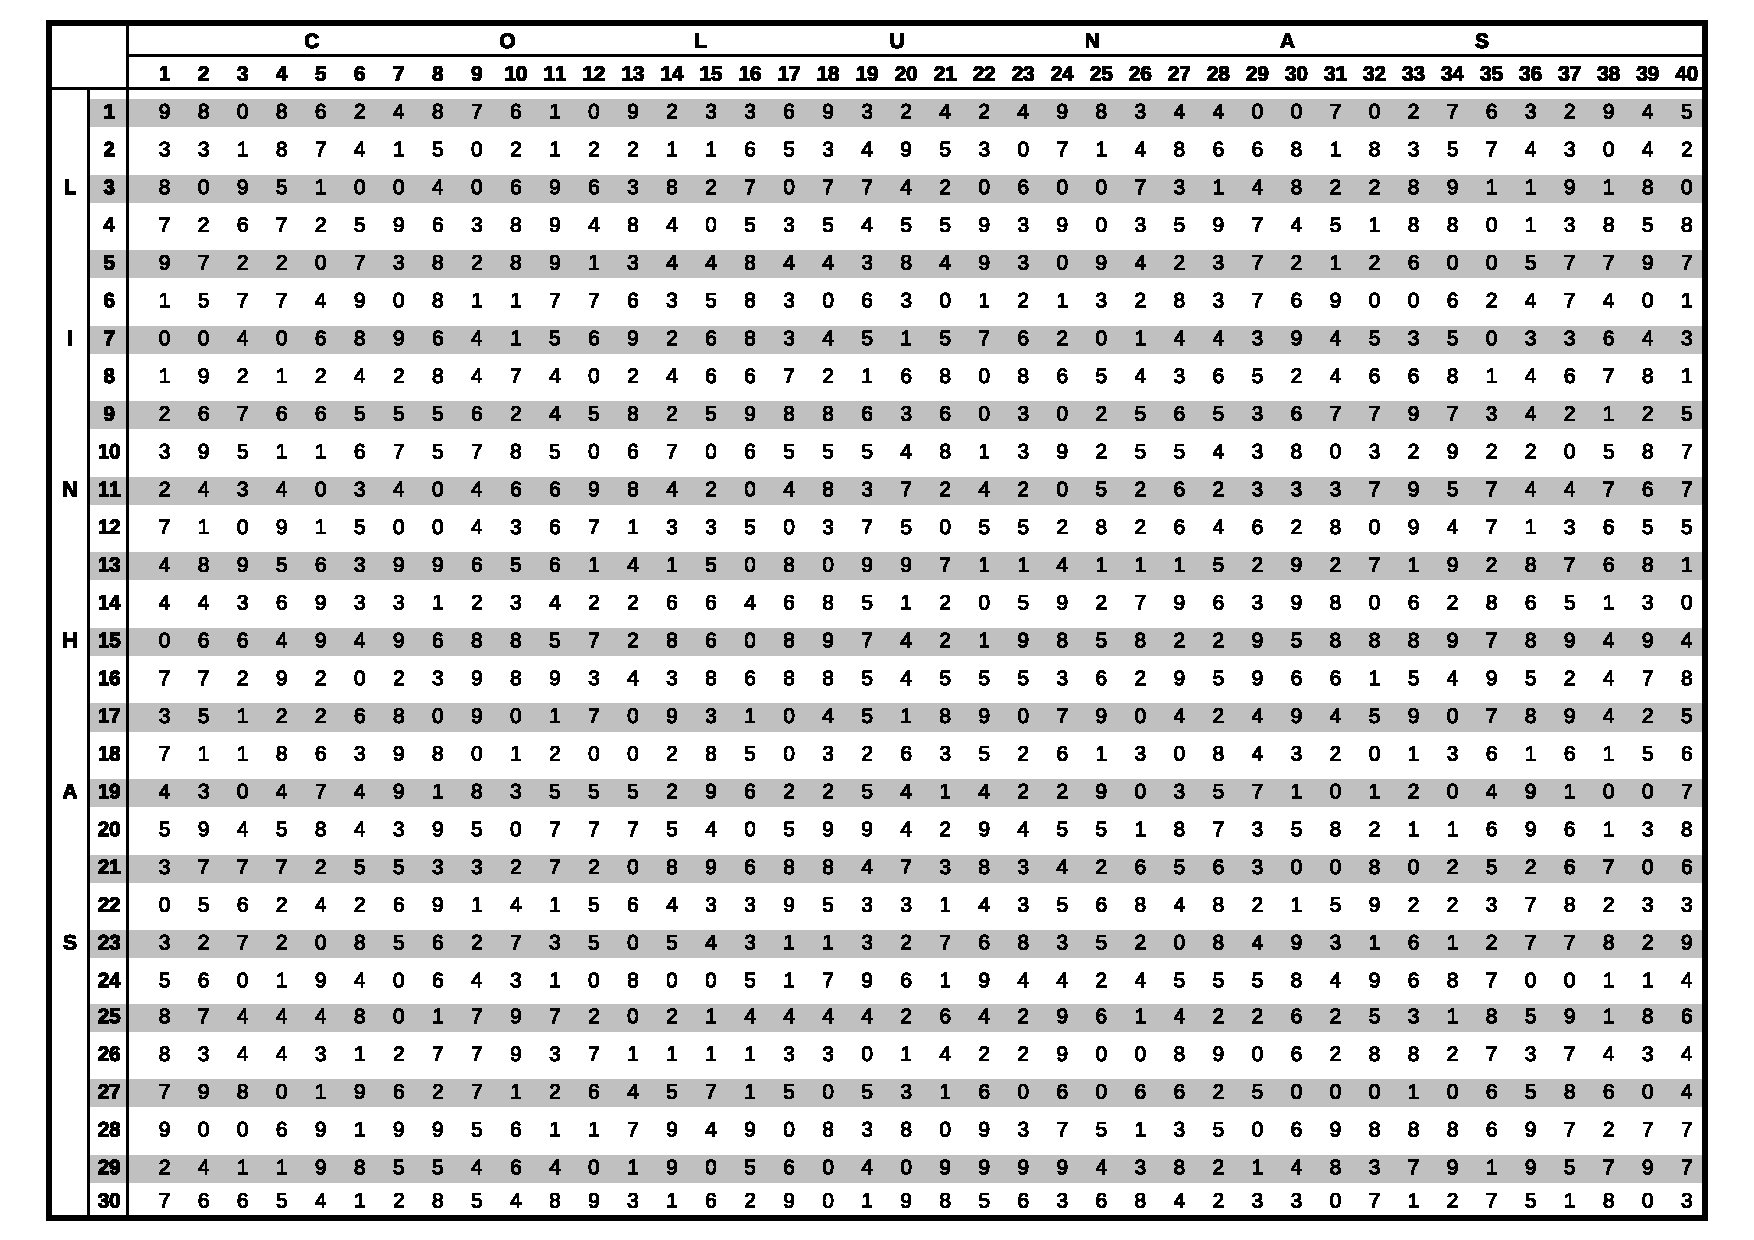
\includegraphics[width=\paperwidth, angle=270]{anexos/quadro_num_aleatorios}
\end{figure}

\part{Pós-textual}
\nosidepicturearea
\usechapterimagetrue

%----------------------------------------------------------------------------------------
%	BIBLIOGRAPHY
%----------------------------------------------------------------------------------------

\chapterimage{heading_bib}
\chapter*{Bibliografia}
\addcontentsline{toc}{chapter}{\textcolor{ocre}{Bibliografia}} % Add a Bibliography heading to the table of contents
\label{cap:bib}

%------------------------------------------------

\section*{Artigos}
\addcontentsline{toc}{section}{Artigos}
\printbibliography[heading=bibempty,type=article]

%------------------------------------------------

\section*{Livros}
\addcontentsline{toc}{section}{Livros}
\printbibliography[heading=bibempty,type=book]

%----------------------------------------------------------------------------------------
%	INDEX
%----------------------------------------------------------------------------------------

\cleardoublepage % Make sure the index starts on an odd (right side) page
\phantomsection
\setlength{\columnsep}{0.75cm} % Space between the 2 columns of the index
\addcontentsline{toc}{chapter}{\textcolor{ocre}{Index}} % Add an Index heading to the table of contents
\printindex % Output the index

%----------------------------------------------------------------------------------------

\end{document}